%%%%%%%%%%%%%%%%%%%%%%%%%%%%%%  IEEEsample.tex
%%%%%%%%%%%%%%%%%%%%%%%%%%%%%%%%%%%%%%%%%
%%%%%%%%%%%%%%%%%%%%%%%    More information: see the header of IEEEtran.sty
%%%%%%%%%%%%%%%%%%%%%%%
%%%%%%%%%%%%%%%%%%%%%%%%%%%%%%%%%%%%%%%%%%%%%%%%%%%%%%%%%%%%%%%%%%%%%%%%%%%%%%%%
%%%%

\documentclass[10pt,twocolumn]{IEEEtran}
%\documentclass[conference]{IEEEtran}

%%%\IEEEoverridecommandlockouts


%% set page size to US letter
\special{papersize=8.5in,11in}
\setlength{\pdfpageheight}{\paperheight}
\setlength{\pdfpagewidth}{\paperwidth}

\usepackage{xspace}
%\newcommand{\Grobner}{Gr\"{o}bner\xspace}

\usepackage{algorithm}
\usepackage[noend]{algpseudocode}



%% \usepackage[vlined,boxed,ruled]{algorithm2e}
%% %%for algorithm2e package, label has to be following caption in the same line!!!
%% \renewcommand{\algorithmcfname}{ALGORITHM}
%%  \SetAlFnt{\small}
%%  \SetAlCapFnt{\small}
%%  \SetAlCapNameFnt{\small}
%%  \SetAlCapHSkip{0pt}
%%  \IncMargin{-\parindent}

%% %% \RequirePackage{times}
%%  \RequirePackage{algorithmic}
%%  \PassOptionsToPackage{boxed}{algorithm}
%%  \RequirePackage{algorithm}
%%  \RequirePackage{multicol}
%% \renewcommand{\algorithmicrequire}{\textbf{Inputs:}}
%% \renewcommand{\algorithmicensure}{\textbf{Outputs:}}
 \DeclareMathAlphabet{\mathtsl}{OT1}{ptm}{m}{sl}

%\def\BibTeX{{\rm B\kern-.05em{\sc i\kern-.025em b}\kern-.08em1
%    T\kern-.1667em\lower.7ex\hbox{E}\kern-.125emX}}

%\newtheorem{theorem}{Theorem}
%\newtheorem{lemma}{Lemma}
%\newtheorem{example}{Example}
%\newtheorem{corollary}{Corollary}

\RequirePackage{amssymb, mathptm}
\usepackage{amsbsy}
\usepackage{amsthm}
\usepackage{graphicx}
\usepackage{helvet}
\usepackage{enumerate}
\usepackage{amsmath}
\usepackage{amsfonts}
\usepackage{graphicx}
\usepackage{multirow}
\usepackage{subfig}
\usepackage{comment}
\usepackage{cases}
\usepackage{xcolor}
\usepackage{epstopdf}
\usepackage[normalem]{ulem}

%%indent in algorithm


%\setcounter{page}{1}


% New command for the table notes.
\def\tabnote#1{{\small{#1}}}

% New command for the line spacing.
\newcommand{\ls}[1]
    {\dimen0=\fontdimen6\the\font
     \lineskip=#1\dimen0
     \advance\lineskip.5\fontdimen5\the\font
     \advance\lineskip-\dimen0
     \lineskiplimit=.9\lineskip
     \baselineskip=\lineskip
     \advance\baselineskip\dimen0
     \normallineskip\lineskip
     \normallineskiplimit\lineskiplimit
     \normalbaselineskip\baselineskip
     \ignorespaces
    }
%\renewcommand{\algorithmicrequire}{\textbf{Input:}}
%\renewcommand{\algorithmicensure}{\textbf{Output:}}

\newcommand{\beq}{\begin{equation}}
\newcommand{\eeq}{\end{equation}}
\newcommand{\beqarr}{\begin{eqnarray}}
\newcommand{\eeqarr}{\end{eqnarray}}
%\newcommand{\ov}{\overline}
\newcommand{\ov}{\bar}
\newcommand{\xor}{\bigoplus}
\newcommand{\Fm}{{\mathbb{F}}}
\newcommand{\myfontsize}{\fontsize{7}{9}\selectfont}


%the following is for space before and after align or other equation environment.

%%
\newtheorem{Algorithm}{Algorithm}[section]
\newtheorem{Definition}{Definition}[section]
\newtheorem{Example}{Example}[section]
\newtheorem{Proposition}{Proposition}[section]
\newtheorem{Lemma}{Lemma}[section]
\newtheorem{Theorem}{Theorem}[section]
\newtheorem{Corollary}{Corollary}[section]
\newtheorem{Conjecture}{Conjecture}[section]
\newtheorem{Problem}{Problem}[section]
\newtheorem{Notation}{Notation}[section]
\newtheorem{Setup}{Problem Setup}[section]

%%%

%%set spacing between table columns
\setlength{\tabcolsep}{3pt}

\begin{document}

%\thispagestyle{empty}
%\pagestyle{empty}

%\ls{1.5}


\title{\Large\textsc{Boolean Gr\"obner Basis Reductions on Datapath Circuits using the Unate Cube Set Algebra}}
\author{Utkarsh Gupta, Priyank Kalla, Vikas Rao \\
Electrical \& Computer Engineering, University of Utah \vspace{-0.2in}
}
%\affiliation{Electrical \& Computer Engineering, University of Utah}
% \email{}    
 
 
\maketitle
\thispagestyle{empty}
% Modified by  K. Kobayashi \maketitle 

%\markboth{MS Proposal by Tim Pruss}{}
\newcommand{\Fq}{{\mathbb{F}}_{q}}
\newcommand{\Fkk}{{\mathbb{F}}_{2^k}}
\newcommand{\Zkk}{{\mathbb{Z}}_{2^k}}
\newcommand{\Ftwo}{{\mathbb{F}}_{2}}
\newcommand{\Fkkx}[1][x]{\ensuremath{\mathbb{F}}_{2^k}[#1]\xspace}
\newcommand{\Grobner}{Gr\"{o}bner\xspace}
\newcommand{\B}{{\mathbb{B}}}
\newcommand{\Z}{{\mathbb{Z}}}
\newcommand{\F}{{\mathbb{F}}}
\newcommand{\G}{{\mathcal{G}}}
\newcommand{\alert}[1]{\textcolor{red}{#1}}

\newcommand{\spec}{{\it Spec}\xspace\ \xspace}
%%%

\newcommand{\debug}[1]{\textcolor{gray}{[ #1 ]}}


%%%%%%%%%%%%%%%%%%%% Include your files here %%%%%%%%%%%%%%%%%%%%%
\begin{abstract}
Recent developments in formal datapath verification make efficient use 
of symbolic computer algebra algorithms for formal verification. The
circuit is modeled as a set of polynomials over Boolean (or
pseudo-Boolean) rings, and  Gr\"obner basis (GB) reductions are
performed over these polynomials to derive a canonical
representation. GB reductions of Boolean polynomials tend to cause
intermediate expression swell (term explosion problem) -- often making
the approach infeasible in a practical setting. To overcome these
problems,  this paper describes a logic synthesis analogue of GB
reductions over Boolean polynomials, using the unate cube set algebra
over characteristic sets. By representing Boolean polynomials as
characteristic sets using Zero-suppressed BDDs (ZBDDs), implicit
algorithms can be efficiently designed for GB-reduction on digital
circuits. We show that imposition of circuit-topology based monomial
orders on ZBDDs enables an implicit implementation of polynomial
division, canceling multiple monomials in one-step. 
%Other recent
%strategies of GB-reduction on circuits can also be implemented
%efficiently on ZBDDs. 
Experiments performed over various finite field
arithmetic architectures demonstrate the efficiency of our 
algorithms and implementations as compared to conventional explicit
methods. 
\end{abstract}

\section{Introduction}

Craig interpolation is a method to construct and refine abstractions
of functions. It finds application in formal verification of hardware
designs and software programs, in logic synthesis of Boolean
functions, and also as a tool in proof complexity theory. It is a
logical tool to extract concise explanations for the infeasibility of
a mutually inconsistent set of statements. Craig
\cite{craig-interpolate} showed that for a valid implication $A
\implies B$, where $A, B$ are first order formulae containing no free
variables, there is a formula $I$ such that $A \implies I$, $I
\implies B$ and the non-logical symbols of $I$ appear in both $A$ and
$B$. The formula $I$ is called the {\it Craig interpolant}, or
interpolant for short. As  
propositional logic also admits Craig interpolation, the formal
verification community has extensively investigated interpolants and
their computation from resolution proofs of CNF-SAT problems. In the
propositional logic domain, the concept is stated with a slight
modification.  

\begin{Definition}\label{def:ci}
Let $(A, B)$ be a pair of CNF formulae (sets of clauses) such that $A
\w B$ is unsatisfiable. Then there exists a formula $I$ such that: (i)
$A\implies I$; (ii) $I \w B$ is unsatisfiable; and (iii) $I$ refers
only to the common variables of $A$ and $B$, i.e. $Var(I) \subseteq
Var(A) \cap Var(B)$. The formula $I$ is called the {\bf interpolant}
of $(A,B)$. 
\end{Definition}

Given the pair $(A, B)$ and their refutation proof, a procedure called
the {\it interpolation system} constructs the interpolant in linear
time and space in the size of the proof \cite{McMillan:CAV03}. As the
abilities of SAT solvers for proof refutation have improved,
interpolants have been exploited as abstractions in various problems
that can be formulated as unsatisfiable instances, e.g. model checking
\cite{McMillan:CAV03}, logic synthesis \cite{roland:bidecomp},
etc. Their use as abstractions have also been replicated in other
(combinations of) theories \cite{McMillan:TACAS04}
\cite{Kapur:SIGSOFT06} \cite{Cimatti:TACAS08} \cite{Griggio:FMCAD11},
etc.  
%These concepts have been applied to various problems in
%automated reasoning. 
%; {\it e.g.} for the theory of linear
%inequality \cite{McMillan:TACAS04}, data-type theories
%\cite{Kapur:SIGSOFT06}, Linear arithmetic and difference logic
%\cite{Cimatti:TACAS08}, Bit-vector theories \cite{Griggio:FMCAD11},
%among others.  


In this paper, we introduce the notion of {\it Craig interpolants in
polynomial algebra over finite fields} ($\Fq$) of $q$ elements, where
$q = p^k$ is a prime power. Given a mutually inconsistent pair of sets
of polynomials with coefficients from $\Fq$ that have no common zeros,
we show that Nullstellensatz over finite fields admits
interpolation. We represent the sets $A, B$ (from Def. \ref{def:ci}) as
{varieties of corresponding ideals}, and prove the existence of
an interpolant for the pair $(A,B)$. In this setting, {\it interpolants
correspond to varieties} -- subsets of the $n$-dimensional affine
space $\Fq^n$ -- and are represented by polynomial ideals, more
precisely, by a {\it Gr\"obner basis of corresponding ideals.}

Intuitively, it should be apparent that polynomial algebra over finite
fields would admit Craig interpolation (a first order theory over
$\Fq$ definitely admits quantifier elimination \cite{gao:qe-gf-gb}).
However, our literature search for interpolants and their computation
with polynomials in arbitrary finite fields did not reveal much prior
work in this area. %turned out to be unsuccessful. 
%There is a need for the theory and algorithms for
%interpolation in this domain. 
Recent years have witnessed
investigations in formal verification, abstraction and synthesis of
datapath circuits with $k$-bit operands, where the problems have been
modeled 
%using algebraic geometry 
over finite fields ($\Fkk$) \cite{pruss:tcad} \cite{xiaojun:hldvt2016}
or over finite integer rings ($\Zkk$) \cite{sivaram:todaes}. 
%Analogous to Boolean
%function decomposition, 
%there is also a need for polynomial (word-level) datapath synthesis
Interpolants can be exploited as abstractions of functions
($f:\Fkk\rightarrow\Fkk$) in this domain, and can make these
approaches practical. Motivated by the above needs, this paper
presents the theory of Craig interpolation in finite fields, and
describes algorithms to compute them.  


{\it Contributions:} Using the extensive machinery of algebraic
geometry in finite fields,
% -- including Nullstellensatz, projections of
%varieties, elimination and extension theory, set operations on ideals
%and varieties, etc. -- 
this paper makes the following contributions: 
1) Formally define the notion of interpolants in polynomial algebra
  over finite fields $\Fq$, and prove their existence in this domain.
2) Derive the relationship of interpolants with elimination ideals,
  and show how to compute them using Gr\"obner bases. 
3) Compute the {\it smallest} interpolant, i.e. the one
  contained in every other interpolant. Analogously, compute the
  {\it largest} interpolant, i.e. the one containing all
  other interpolants. 
4) Count the total number of all possible interpolants.
5) We show how all interpolants can be enumerated in
$\mathbb{F}_2$. However, as it is impractical to explore all possible
interpolants, we present an algorithm to heuristically enumerate a few
interpolants (explore the interpolant lattice): beginning with the
smallest, progressively visiting larger ones,   and terminating at the
largest interpolant.  

{\it Paper Organization:} The following section briefly reviews prior
work in Craig interpolation in various theories, and contrasts it
against the concepts presented in this paper. Section \ref{sec:prelim} 
describes the preliminary concepts of algebraic geometry and Gr\"obner
bases in finite fields. Section \ref{sec:theory} describes the theory
of interpolation in finite fields and shows how they can be computed
using the Gr\"obner basis algorithm. Section \ref{sec:alg} describes
techniques and an algorithm to enumerate the interpolants. 
%All the concepts are also demonstrated by means of
%examples. \debug{Section \ref{sec:dis} compares our results against
%interpolant-classification in propositional logic. --  we will see
%about this} 
Section \ref{sec:exp} describes some of our experiments with unsat
instances to generate the interpolants. Section
\ref{sec:conc} concludes the paper.  Some of the proofs of the
theorems and lemmas are omitted from the main body of the manuscript
and are included in an appendix. 

%The omitted proofs of
%the theorems and lemmas are contained in an appendix.

\vspace{-0.1in}
\section{Review of Previous Work}
In the past decade or so, there has been an explosion in the study,
classification and application of interpolants. In abstraction-based
model checking, interpolants are used as over-approximate image
operators \cite{McMillan:CAV03}. In Boolean function decomposition,
given a function $F(A, B, C)$ with support variables partitioned into
disjoint subsets $A, B, C$, it is required to decompose $F = G(A, C)
\odot H(B,C)$, where $\odot$ denotes the Boolean $\vee, \wedge,
\oplus$ operations. The existence of such a 
decomposition with the given variable partition is formulated as a
unsatisfiability checking problem. Craig interpolants can then be used
to compute $G, H$ \cite{roland:bidecomp}
\cite{roland:ashenhurst}. 
%Conceptually, these problems 
%have quantifiers and interpolants can be used in lieu of the more
%expensive quantifier elimination. 
In proof complexity, interpolants have been used as a tool to derive 
lower bounds; {\it e.g.} by reasoning that if $A\implies B$ does not
have a simple interpolant, then it cannot have a simple proof
\cite{pudlak:ci}. The authors in \cite{PudlakPCFA1998} present
an interpolation theorem for Nullstellensatz refutations and the
polynomial calculus \cite{CEI:stoc-96} which can then be used for
proving lower bounds. 

The use of interpolants as abstractions has also been replicated in
other combinations of theories. For example, the theory of linear
inequality \cite{McMillan:TACAS04}, data-type theories
\cite{Kapur:SIGSOFT06}, linear arithmetic and difference logic
\cite{Cimatti:TACAS08}, bit-vector SMT theories
\cite{Griggio:FMCAD11}, etc., are just a few of the many instances
of the usage of interpolation in various domains outside of purely
propositional logic. The aforementioned works derive interpolants from
resolution proofs obtained from SAT/SMT-solvers
(\cite{Cimatti:TACAS08}), or generate them by solving constrains
in the theories of linear arithmetic with uninterpreted functions
(\cite{Rybalchenko:VMCAI-2007}),  or exploit their connection to
quantifier elimination (\cite{Kapur:SIGSOFT06}), etc. As an 
alternative to interpolation, \cite{Kovacs2009} suggests the use of
local proofs and symbol eliminating inferences for invariant
generation.  
%%  to interpolation based on symbol
%% elimination inferences is presented in  which can be 
%% applied even for theories not having the interpolation property. 
However, the problem has been insufficiently investigated over
polynomial ideals in finite fields from an algebraic geometry
perspective. 


The works that come closest to ours are by Gao {\it et al.}
\cite{gao:qe-gf-gb} and \cite{gao:gf-gb-ms}. While they do not
address the interpolation problem per se, they do describe important
results of Nullstellensatz, projections of varieties and quantifier
elimination over finite fields that we extensively utilize in this
paper.  

The work of \cite{dsilva:vmcai2010} classifies (orders) the
interpolants according to their logical strength for model 
checking. They present a labeled interpolation system built on the
resolution proof where each vertex of the proof is annotated with
partially ordered labels.  Interpolants generated from different sets
of labels have the same  order of strength as the order of the labels.
This way a (sub-)lattice of interpolants is generated with the
smallest interpolant being the same as obtained from the McMillan's
system ($L_M$) \cite{McMillan:CAV03} and the largest being the
complement of inverse of $L_M$. In contrast, we present a method for
polynomials in $\F_2$ that can generate the complete lattice of
interpolants with the absolute smallest and   absolute largest
interpolants. The labeled interpolation system of
\cite{dsilva:vmcai2010} is generalized  to support  propositional
hyper-resolution proofs \cite{Weissenbacher2012}. 
% They show how to transform a refutation proof to generate
% interpolants of various strengths. 
More recently, \cite{rummer:fmcad2013} presents the notion of
interpolation abstraction, and describes a semantic framework for
exploring interpolant lattices. In contrast to these works that
qualitatively order the interpolants w.r.t. a given application
(e.g. model checking),  we describe a method to explore interpolants
based on the cardinality of the zero-sets of polynomial ideals, which
in turn corresponds to the size of the abstraction.  


%\section{Preliminaries: Notation and Background}
\section{Background: \Grobner Basis Reduction and Canonical Representations}
\label{sec:prelim}

%This section provides a brief description of the fundamental concepts of: 
%%i) commutative algebra including polynomial rings, polynomial division, ideals, 
% Gr\"obner basis and their application in verification of circuits;
%ii) the algebra of unate cube sets; and iii) the use of ZDDs as an
%implicit set representation for manipulation of Boolean polynomials.

%\subsection{Computer Algebra}

% i.e., $G = GB(J) \Leftrightarrow\  \forall f \in J : f \neq 0 \ \exists g_i \in G :
%lm(g_i)\mid lm(f)$. 

\par Let $\B =\{0,1\}$ denote the Boolean domain, $\F_2$ the finite field
of 2 elements ($\B \equiv \F_2$), and $R = \F_2[x_1, \dots, x_n]$
the  polynomial ring over variables $x_1, \dots, x_n$ with
coefficients in $\F_2$.  
%Since $\Fkk$ is a $k$-dimensional extension of $\F_2$, we
%have that $\Fkk \supset \F_2$ and all $\Fkk (k \geq 1)$ are of
%characteristic 2. 
Operations in $\F_2$ are performed $\pmod{ 2}$, so $-1=+1$ in
$\F_2$. We will use $+ ,\cdot$ to denote addition and multiplication in
$R$, and $\neg, \vee, \wedge$ and $\oplus$ to denote Boolean negation,
OR, AND and XOR operations, respectively. 

A polynomial $f \in R$ is written as a finite sum of terms 
$f = c_1 X_1 +  c_2 X_2 + \dots + c_t X_t$.  Here $c_1, \dots, c_t$
are coefficients and $X_1, \dots, X_t$ are monomials, i.e. power
products of the type $x_1^{e_{1}}\cdot x_2^{e_{2}}\cdots x_n^{e_{n}}$, 
$e_i \in \Z_{\geq  0}$. To systematically manipulate the
polynomials, a monomial order $>$ (also called a term order) is
imposed on the ring. This order $>$ is a total order and a well
order on all the monomials of $R$ such that multiplication by a
monomial preserves the order\footnote{Lexicographic ({\it lex}) and
  degree-lexicographic ({\it deglex}) are examples of such permissible
  monomial orders.}. All polynomials in $R$ are represented using
$>$. Subject to $>$, when a polynomial is written as 
$f = c_1 X_1 +  c_2 X_2 + \dots + c_t X_t$ 
 such that  $X_1 >X_2 > \dots >  X_t$, we call  $lt(f) = c_1 X_1,
 ~lm(f) = X_1, ~lc(f) = c_1$, the {\it leading   term}, {\it   leading
   monomial} and {\it   leading coefficient} of $f$,
 respectively, with $lt(f) = lc(f)\cdot lm(f)$. 
We also denote tail($f$) = $f - lt(f) = c_2X_2 + \dots + c_t X_t$. 
In this work, we are mostly concerned with terms ordered
lexicographically ({\it lex}). 

\begin{Definition} [Boolean Polynomial]
Let $f = c_1 X_1 + \dots + c_t X_t$ be a polynomial in
$\F_2[x_1,\dots,x_n]$ such that the coefficients $c_i \in \{0, 1\}$,
and monomials $X = x_1^{e_{1}}\cdot x_2^{e_{2}}\cdots x_n^{e_{n}}, e_i
\in \{0,1\}$. 
Then $f$ is called a {\bf Boolean polynomial}. For Boolean polynomials
$lt(f) = lm(f)$. 
\end{Definition}

% \textcolor{red}{\begin{Definition} [Pseudo-Boolean Polynomial]
% Let $f = c_1 X_1 + \dots + c_t X_t$ be a polynomial
% such that the coefficients $c_i \in \mathbb{Z}$,
% and monomials $X = x_1^{e_{1}}\cdot x_2^{e_{2}}\cdots x_n^{e_{n}}, e_i
% \in \{0,1\}$. 
% Then $f$ is called a {\bf pseudo-Boolean polynomial}.
% \end{Definition}}

A gate-level circuit can be modeled with Boolean polynomials, where
every Boolean logic gate operator is mapped from $\B$ to a polynomial
function over ${\mathbb{F}}_2$: 

{\small
\begin{equation}
\label{b2poly}
\begin{split}
z ~ =  ~ \neg a ~ & \mapsto ~ z+a+1 \pmod 2  \\
z ~ =  ~ a \wedge b ~ & \mapsto ~ z+a\cdot b \pmod 2\\
z ~ =  ~ a \vee b ~ & \mapsto ~ z+a+b+a\cdot b \pmod 2 \\
z ~ =  ~ a \oplus b ~ & \mapsto ~ z+a+b \pmod 2 
\end{split}
\end{equation}
}

% Using this mapping a Boolean function, say $z = a \vee b$,  
% can be written as the boolean polynomial, $f:z + a\cdot b + a + b$. 
% The solutions to $f = 0$ provide the valid enumerations of  the output and input variables.
%  In this case, $f$ is 0, when $(z,a,b) = \{000,110,101,111\}$  

{\bf Polynomial reduction via division:} Let $f, g$ be polynomials. If
$lm(f)$ is divisible by $lm(g)$, then we say that $f$ {\it is
  reducible to} $r$ modulo $g$, denoted $f
\stackrel{g}{\textstyle\longrightarrow} r$, where $r = f - {lt(f)
  \over   lt(g)} \cdot g$. This operation forms the core operation of
polynomial division algorithms and it has the effect of canceling the
leading term of $f$. 
Similarly, $f$ can be {\it reduced 
w.r.t. a set of polynomials}  $F = \{f_1, \dots, f_s\}$ to obtain a
remainder $r$. This reduction is denoted as $f \stackrel{F} {\textstyle
  \longrightarrow}_+ r$, and the remainder $r$ has the property that
no term in $r$ is divisible (i.e. cannot be canceled) by the leading
term of any polynomial $f_i$ in $F$. Algorithm~\ref{algo:mv_reduce}
(Alg. 1.5.1 from \cite{gb_book}) depicts the procedure to perform this
classical reduction that cancels one monomial in every iteration of
the while-loop.   

\begin{algorithm}[H]
 \caption{Multivariate Reduction of $f$ by $F=\{f_1,\dots,f_s\}$}
 \label{algo:mv_reduce}
 \begin{algorithmic}[1]
 % \Procedure{$multi\_variate\_reduce$}{$f, f_1, \dots, f_s \in \F[x_1, \dots, x_n], f_i\neq 0$}
 \Procedure{$multi\_variate\_reduce$}{$f, \{f_1, \dots, f_s\}, f_i\neq 0$}
 % \ENSURE $u_1,\dots, u_s, r$ s.t. $f = \sum f_i u_i+r$ where $r$ is
 % reduced w.r.t. $F = \{f_1,\dots, f_s\}$ and max($lp(u_1)lp(f_1), \dots, lp(u_s)lp(f_s), lp(r)$) = $lp(f)$
 \State $u_i \gets 0; ~r \gets 0; ~h \gets f $ 
 \While {  $h \neq 0$ }
 \If{ $\exists i$ s.t. $lm(f_i) ~|~ lm(h)$}
 \State choose $i$ least s.t. $lm(f_i) ~|~ lm(h)$
 \State $u_i = u_i + \frac{lt(h)}{lt(f_i)}$
 \State $h = h - \frac{lt(h)}{lt(f_i)} f_i$
 \Else
 \State $r = r+ lt(h)$
 \State $h = h - lt(h)$
 \EndIf
 \EndWhile
 \State \Return $(\{u_1,\dots,u_s\} , r)$
 \EndProcedure
 \end{algorithmic}
 \end{algorithm}

% The algorithm initializes $h$ with the polynomial $f$ and cancels its
% leading term by some  polynomial $f_i \in F$. If the leading term
% $lt(h)$ cannot be canceled by any $lt(f_i)$, then it is added to the  
% remainder $r$ and the process is repeated until all the terms in $h$ are analyzed. 

{\bf Polynomial ideals:} Given a set of polynomials $F = \{f_1, \dots,
f_s\}$ from the ring $R = \mathbb{F}_2[x_1,\dots, x_n]$, the ideal 
generated by $F$ is $J = \langle F\rangle \subseteq R$:
\begin{align}
J = \langle f_1, \dots, f_s \rangle =
\{h_1\cdot f_1+\dots+h_s\cdot f_s: ~h_1,\dots,h_s \in R\},
\end{align}
where the polynomials $f_1,\dots,f_s$ are called the generators (or
basis) of the ideal. 


For a binary variable $x_i$, we have $x_i^2 = x_i$. Therefore, the
polynomial $x_i^2 - x_i$ vanishes over $\Ftwo$, and we call it a
vanishing polynomial. While manipulating Boolean polynomials it is
essential to ensure this indempotency by reducing the polynomials
modulo (the ideal of) all vanishing polynomials $\langle
x_1^2-x_1,\dots,x_n^2-x_n\rangle$. Therefore, %mathematically speaking
we essentially operate on the quotient ring of $\Ftwo[x_1,\dots,x_n]$
modulo the ideal of vanishing polynomials, i.e. %denoted 
over $\Ftwo[x_1,\dots,x_n]/\langle x_1^2-x_1,\dots,x_n^2-x_n\rangle$. 
Then Boolean polynomials are exactly the canonical representatives of
residue classes in the aforementioned quotient ring. A significant
benefit of using a Boolean data-structure such as ZDDs is that the
reduction $x_i^2 = x_i$ is performed implicitly by the
data-structure. 
%, thus improving symbolic computation. Therefore, 
For this reason, in the sequel we {\it omit explicit mention} of
reduction modulo the vanishing polynomials 
% for manipulation of Boolean polynomials, 
and it should be assumed that the reduction $x_i^2 = x_i$
is always performed. 
%It should be clear that in the ZDD-based framework, all
%computations implicitly result in a Boolean polynomial where

{\bf \Grobner basis of ideals:} An ideal $J$ may have many different sets
of generators, i.e. it is possible to have  $J = \langle f_1, \dots,
f_s\rangle = \langle h_1,\dots, h_r\rangle = \dots = \langle g_1,
\dots, g_t \rangle$. A \Grobner basis $G$ of ideal $J$ is one such set
of polynomials $G = GB(J) = \{g_1, \dots, g_t\}$ with many important
properties that allow to solve many polynomial decision questions. 
%A
%\Grobner basis is essentially a canonical representation of the ideal.   

\begin{Definition}[Gr\"obner basis \cite{gb_book}]
\label{def:gb}
%$\bf{\left[Gr\ddot{o}bner\ Basis\right]}$ 
For a monomial ordering $>$, a set  of non-zero polynomials $G =
\{g_1,g_2,\dots,g_t\}$ contained in an ideal $J$, is called a
Gr\"{o}bner basis of $J$ iff 
$\forall f \in J$, $f\neq 0$, there exists $g_i \in 
\{g_1,\dots, g_t\}$ such
that $lm(g_i)$ divides $lm(f)$; i.e., 
$G = GB(J) \Leftrightarrow\  \forall f \in J : f \neq 0, \ \exists g_i \in G :
lm(g_i)\mid lm(f)$. 

\end{Definition}


\par Gr\"obner basis $G$ of an ideal $J = \langle
f_1,\dots,f_s\rangle$ is computed using the Buchberger's
algorithm~\cite{buchberger_thesis}, 
%also given in textbooks \cite{ideals:book} \cite{gb_book}, 
reproduced in Alg. \ref{alg:gb}.

\begin{algorithm}
\caption {Buchberger's Algorithm}
\label{alg:gb}
\begin{algorithmic}[1]
 \Require {$F = \{f_1, \dots, f_s\}$}
 \Ensure  {$G = \{g_1,\dots ,g_t\}$} %, a Gr\"{o}bner basis \\
  \State $G:= F$;
  \Repeat
    \State $G' := G$
    \For {each pair $\{f_i, f_j\}, i \neq j$ in $G'$}
      \State $Spoly(f_i, f_j) \stackrel{G'}{\textstyle\longrightarrow}_+h$ 
      \If {$h \neq 0$} \State $G:= G \cup \{h\}$ \EndIf
    \EndFor
%\hspace{0.2in}  $G(x):=G(x) / x$
  \Until $G = G'$
\end{algorithmic}
\end{algorithm}


% The algorithm initializes the set $G$ with the given generators of $J$
% $i.e.$ $\{f_1,\dots,f_s\}$. Then it takes pairs of polynomials
% ($f_i,f_j$) from the basis and computes their S-polynomial
% $Spoly(f_i,f_j)$:
% algorithm is based on the computation of $Spoly$ of pairwise combination of polynomials 
%in $G$ using the following formula,
In the algorithm,
\begin{equation}
\label{spoly}
\begin{split}
Spoly(f_i,f_j) = \frac{L}{lt(f_i)}\cdot f_i - \frac{L}{lt(f_j)}\cdot f_j
\end{split}
\end{equation}
where $L = LCM(lt(f_i),lt(f_j))$. 
% The $Spoly(f_i,f_j)$ is then reduced
% $w.r.t.$ the polynomials in $G$ to obtain remainder $h$. If $h$ is
% non-zero, it is added to $G$. The process is repeated for all unique
% polynomial pairs, including those generated by the newly added
% elements $h$. The algorithm terminates when there are no new non-zero
% $h$ generated from the set $G$. $Spoly(f_i,f_j)\xrightarrow{G}_+h$
% reductions cancel the leading terms of polynomials $\{f_i,f_j\}$, and
% generate polynomials $h$ with new leading terms, providing additional
% information regarding the ideal.  

An important property of a \Grobner basis $G$ is that reduction of a
polynomial $f$ modulo $G$ is essentially unique. 


\begin{Theorem} [\Grobner Basis Reduction, Thm. 1.9.1 in
      \cite{gb_book}]
\label{thm:gbr}
%$\bf{\left[Gr\ddot{o}bner\ Basis\ Reduction\right]}$ : 
Let $G=\{g_1,\dots,g_t\}$ be a \Grobner basis of ideal $J$, and let $f$
be another polynomial.  The reduction
of $f$ modulo $G$, denoted $f\xrightarrow{G}_+r$, is called the
{\bf \Grobner basis reduction (GBR)} of $f$. The remainder $r$
so obtained by GBR of $f$ is a {canonical expression
modulo $G$}.  
\end{Theorem}

In other words, for {any polynomial} $f$, if $f\xrightarrow{G}_+r_1$
and $f\xrightarrow{G}_+r_2$, then $r_1 = r_2=r$. 
%% The \Grobner basis
%% also provides a decision procedure for ideal membership: To test if
%% any polynomial $f \in J$, we compute $G = 
%% GB(J)$ and check if $f \xrightarrow{G}_+ 0$? 
The remainder $r$ is sometimes also called the {\it normal form} of
$f$ w.r.t. $G$. The canonicity of $r$ (modulo $G$) can be exploited
for equivalence checking of digital circuits. 


%{Verification Formulation}

\begin{Proposition}\label{prop:verif}
Given a circuit $C$, we can represent all the gates using (Boolean)
polynomials $F = \{f_1, \dots, f_s\}$ in $\F_2[x_1,\dots,x_n]$ by
means of Eqn. (\ref{b2poly}), and generate ideal $J  = \langle F \rangle$. Let
$z_i, ~i = 0,\dots,{k-1}, (z_i \in \{x_1,\dots,x_n\})$ denote one-bit of the
$k$-bit primary output variables   
of the circuit.  Compute a \Grobner basis $G = GB(J) =
\{g_1,\dots,g_t\}$ for the polynomials of the circuit, and perform the
GBR $z_i\xrightarrow{G}_+ r_i$ for all $0\leq i<k$. Then all $r_i$'s
are a canonical representation and can be used for formal
verification/equivalence checking. 
\end{Proposition}

To derive the canonical representation $r_i$, it is required to
compute a \Grobner basis $G$ of the ideal generated by the polynomials
of the circuit. Buchberger's algorithm for computation of a Gr\"obner
basis exhibits high complexity. 
% In general, the worst-case \Grobner
% basis complexity is doubly-exponential in the input data
% \cite{Dube:gb-complexity}. However, over ideals that have a finite
% number of solutions, the complexity is single exponentially
% bounded. Particularly 
Over finite fields $\Fq$ of $q$ elements ($q =
2$ in our case), the complexity is bounded by $q^{(O(n))}$, where $n$
is the number of variables \cite{gao:gf-gb-ms}. This complexity still
needs to be overcome. The work of \cite{lv:tcad2013} showed that for
formal verification of combinational circuits, the expensive GB
computation can be avoided altogether, due to the following results. 

\begin{Lemma}[Product Criterion \cite{productc:1979}]
\label{prod_criteria}
%${\bf \left[Product \ Criterion\right]}$ : 
For two polynomials $f_i,f_j$  in any polynomial ring $R$, if the
equality $lm(f_i)\cdot lm(f_j) = LCM(lm(f_i),lm(f_j))$ holds, i.e. if
$lm(f_i)$ and $lm(f_j)$ are relatively prime, then 
$Spoly(f_i,f_j) \xrightarrow{G}_+ 0$.  
\end{Lemma}
 

Using this criterion we can say that when the leading terms of {\it all
polynomials in the basis} $F = \{f_1, \dots, f_s\}$ are relatively
prime, then all $Spoly(f_i,f_j)  \xrightarrow{G}_+ 0$.  As no new
polynomials are generated in Buchberger's algorithm, $F$ is already a
\Grobner basis ($F = GB(J)$). For a combinational
circuit $C$, a specialized term order $>$ can always be derived by
analyzing the circuit topology which ensures such a property
\cite{wienand:cav08} \cite{lv:tcad2013}:  

\begin{Proposition} \label{prop:top-order}
(From \cite{lv:tcad2013}) Let $C$ be an arbitrary combinational
  circuit. Let $\{x_1, \dots, x_n\}$ denote the set of all variables
  (signals) in $C$. Starting from the primary outputs, perform
  a {\it reverse topological traversal} of the circuit and order the
  variables such that $x_i > x_j$ if $x_i$ appears earlier in the
  reverse topological order. Impose a {\it lex} term order $>$ to
  represent each gate as a polynomial $f_i$, s.t. $f_i = x_i +
  tail(f_i)$. Then the set of all polynomials  $\{f_1, \dots, f_s\}$
  forms a Gr\"obner basis G, as $lt(f_i)=x_i$ and $lt(f_j)=x_j$ for
  $i\neq j$ are relatively prime. This term order $>$ is called the 
  {\bf Reverse Topological Term Order (RTTO)}.
\end{Proposition}

Imposition of RTTO on the polynomials of the circuit has the effect of
making every gate output variable $x_i$ a leading term of
$f_i$. Since every gate output is unique, $lm(f_i)=x_i, lm(f_j)=x_j$
become relatively prime. As a result, the set $F$ is already a GB
($G=F$), the explosive GB computation is avoided, and verification is
performed solely by the canonical GB-reduction: $z_i \xrightarrow{G}_+r_i$. 
Note that as $f_i = x_i + \text{tail}(f_i)$, RTTO ensures that
every variable $x_j$ that appears in $\text{tail}(f_i)$ satisfies
$x_i>x_j$. Moreover, the remainder $r_i$ comprises only primary inputs
of the circuit. These properties will be exploited in our algorithms.

% \vspace{-0.1in}
\begin{figure}[!h]
\begin{minipage}[t]{3.25in}
% \vspace{0pt}
\centerline{
%\includegraphics[scale=0.3]{../figures/2bitmultiplier.eps}
\includegraphics[scale=0.5]{figures/2bitmultiplier_gates.pdf}
}
\caption{\small A 2-bit modulo Multiplier circuit. 
% The gate $\otimes$ is an
%   AND-gate, and $\oplus$ is an XOR-gate; i.e. $\times, +$ modulo 2,
%   respectively.
  } 
\label{fig:mul2bit}
\end{minipage}
\hfill
\begin{minipage}[t]{3.25in}
\vspace{0pt}
%{\small
\begin{align*}
f_1: c_0+a_0 \cdot b_0, \ lm=c_0; ~~~f_2: c_1+a_0 \cdot b_1, \ lm=c_1 \nonumber \\
f_3: c_2+a_1 \cdot b_0, \ lm=c_2; ~~~f_4: c_3+a_1 \cdot b_1, \ lm=c_3 \nonumber \\
f_5: r_0+c_1 + c_2 , \ lm=r_0; ~~~f_6: z_0+c_0 + c_3, \ lm=z_0\nonumber
\end{align*}
\vspace{-0.35in}
\begin{center}
$f_7: z_1+r_0 + c_3, \ lm=z_1$ % \nonumber 
\end{center}
%}
\caption{\small {Polynomials of the circuit under RTTO constitute a GB.
}} 
\label{fig:rel_prime_lt}
\end{minipage}

\end{figure}

%\vspace{-0.1in}
\begin{Example}
\label{ex1}
{\bf Demonstration of the approach:} Consider the circuit given in
Fig. \ref{fig:mul2bit}. 
%Perform a ``reverse topological traversal'' of the circuit. 
Impose RTTO on the circuit. The primary outputs $z_0, z_1$ are both at
level-0, variables $r_0, c_0, c_3$ are at level-1, ~$c_1, c_2$ are at
level-2, and the primary inputs $a_0, a_1, b_0, b_1$ are at
level-3. Order the variables $\{z_0 > z_1\} > \{r_0 > c_0 > c_3\} >
\{c_1 > c_2\} > \{a_0 > a_1 > b_0 > b_1\}$. Using this variable order,
we impose a {\it lex} term order on the monomials. Then all the
polynomials extracted from the circuit have relatively prime leading
terms, as shown in Fig. \ref{fig:rel_prime_lt}, and $G =F = \{f_1, \dots,
f_7\}$ forms a GB. 

Then the GBRs $z_1\xrightarrow{G}_+ a_0\cdot b_0 + a_1\cdot b_1$ and
$z_0\xrightarrow{G}_+a_0\cdot b_1+a_1\cdot b_0 + a_1\cdot b_1$ are
canonical expressions (Boolean polynomials) of the output bits and can
be used for equivalence checking.
\end{Example}


% We will now show how to efficiently implement this GBR
% $z_i\xrightarrow{G}_+r_i$ on circuits by exploiting the implicit set
% representation ZDDs under the imposition of RTTO. 



\section{Unate Cube Sets \& Boolean Polynomials}
\label{sec:unate}

A Boolean {\it variable} represents a dimension of the Boolean space
$\B^n$, and a {\it literal} 
is an instance of a variable $x_i$ or its 
complement $\neg x_i$. A {\it cube} is a product of literals
which denotes a point or a set of points in the Boolean space. A {\it
  cube set} 
consists of a collection of cubes, each of which is a combination of
literals. {\it Unate cube sets} allow for the use of only positive
literals, not negative/complemented literals. 
%Each cube in a unate
%cube set represents a combination, and each literal represents an
%object selected in the combination.

When cube sets are used to represent Boolean functions, they are
usually {\it binate} cube sets containing negative literals. In binate
cube sets, literals $x_i$ and $\neg x_i$ represent $x_i = 1$ and $x_i = 0$,
respectively; while the absence of a literal implies a {\it don't
  care.} In unate cube sets, literal $x_i$ implies $x_i = 1$ whereas
its absence implies $x_i = 0$. For example, the cube set $\{a,
bc\}$ corresponds to points $(abc): \{111, 110, 101, 100, 011\}$ in
the binate cube set representation, whereas it represents $(abc):
\{100, 011\}$ in the unate cube set representation.

Each monomial of a Boolean polynomial can be viewed as a unate cube --
a product of positive literals -- and a Boolean polynomial as a unate
cube set. Then the GBR $z_i\xrightarrow{G}_+ r_i$ can be interpreted
as %(Boolean) algebra 
operations over unate cube sets, 
%resembling a classical logic synthesis problem, 
as shown below. Let us (re)consider the one-step
division for Boolean polynomials: $f\xrightarrow{g} r$. This division
can be interpreted as:



 \begin{align}
\label{eqns:reduce}
f \xrightarrow{g} r & = f - {{lt(f)} \over {lt(g)}} \cdot g \\
& = ~ f - {{lm(f)} \over {lm(g)}} \cdot g; ~~( ~lt(f)=lm(f))\\ 
& = f + {{lm(f)} \over {lm(g)}} \cdot g; ~~~(-1 = +1 \pmod{ 2})\\
& = f \oplus {{lm(f)} \over {lm(g)}} \cdot g; ~~( as ~+ \pmod{2} =
\oplus) \label{eqns:reduce1}
\end{align}



%% {\small
%% \begin{equation}
%% \label{logic_syn}
%% \begin{split}
%% f \xrightarrow{g} r ~  = & ~ f - {{lt(f)} \over {lt(g)}} \cdot g ~ =  ~ f - {{lm(f)} \over {lm(g)}} \cdot g \\
%% = & ~ f + {{lm(f)} \over {lm(g)}} \cdot g ~ =  ~ f \oplus {{lm(f)} \over {lm(g)}} \wedge g
%% \end{split}
%% \end{equation}
%% }

% $$f \xrightarrow{g} r  = f - {{lt(f)} \over {lt(g)}} \cdot g 
% = ~ f - {{lm(f)} \over {lm(g)}} \cdot g; ~~(\text{coeff. 0,1;}
% ~lt(f)=lm(f))
% $$

% $$= f + {{lm(f)} \over {lm(g)}} \cdot g = f \oplus {{lm(f)} \over
%   {lm(g)}} \wedge g \label{eqns:reduce1}
% $$

%We can replace $lt(f)$ with $lm(f)$ as coefficients are either 0 or
%1. 
Notice that ${{lm(f)} \over {lm(g)}}$ is a unate product of 
literals. i.e. a unate cube. The $\oplus$ operation cancels common
cubes from $f$ and ${{lm(f)} \over {lm(g)}}\cdot g$. The $\cdot$
operation models the modulo 2 product, where the partial products are
added using the $\oplus$  operation. Therefore, we
will implement the reduce operation $f\xrightarrow{g} r$ for Boolean
polynomials as $r = f \oplus {{lm(f)} \over {lm(g)}} \cdot g$ using
an implicit representation particularly suited for such unate cube
operations, i.e. ZDDs.  

\subsection{Zero Suppressed Binary Decision Diagrams (ZDDs) for
  Boolean Polynomials}

% A Binary Decision Diagram is a directed graph with two terminal nodes 0 and 1. 
% Each node in the diagram has two edges, solid edge (1-edge) and dotted edge (0-edge). 

Binary decision diagrams (BDDs) \cite{BRYA86} and
their variants 
%such as OKFDDs \cite{drechsler:dac94} and ADDs \cite{add} 
have been used as implicit representations for solving many
Boolean and pseudo-Boolean optimization problems. Zero-suppressed BDDs
\cite{zbdd} are another variant of BDDs that were designed to
efficiently manipulate ``sets of combinations''. A ZDD is obtained
from an ordered BDD by: i) eliminating those vertices whose 1-edge
(then-edge) is incident on the 0-terminal; and ii) merging isomorphic
subgraphs. Subject to the given variable order, a ZDD represents a 
Boolean function canonically. Just as with BDDs, every node in a ZDD
is assigned an index, which corresponds to the variable order imposed
on the diagram. For a detailed description of ZDDs and
their capabilities for solving logic optimization and sparse
combinatorial problems, the reader is referred to \cite{zbdd} and
\cite{zbdd_unate}. 

\begin{figure}[hbt]
\centering
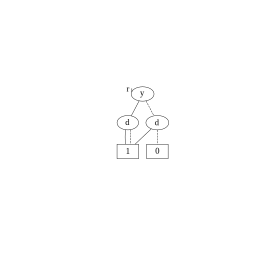
\includegraphics[scale=1]{figures/r1_clean.pdf}
\caption{ZDD for the polynomial $r_1 = yd + y + d$.}
\label{r1}
\end{figure}

In \cite{zbdd_unate}, {\it Minato} demonstrated that ZDDs are an
efficient data-structure for implicit manipulation (algebra) of unate
cube sets. Fig.~\ref{r1} depicts a ZDD for the unate cube set
$\{yd,y,d\}$ with the variable order  $y > d$. The paths beginning
from the root node $y$ and terminating in the 1-terminal node
correspond to the cubes of the set. A variable is present in a cube if
its 1-edge lies on the path; otherwise it is absent from the cube
if its 0-edge lies on the path. 
%Since a monomial of a Boolean
%polynomial is a unate cube, we can interpret a Boolean polynomial as a
%set of unate cubes; and each monomial (cube) as a set of
%variables. 
Consequently, the ZDD of Fig.~\ref{r1} can be construed to
represent the Boolean polynomial $r_1 = yd + y +d$. {\it Minato} has
shown (\cite{zbdd}\cite{zbdd_unate}) how the set union, intersection and
difference operations can be implemented recursively on the ZDDs, 
and they have been implemented using the {\it ite-operator} in
decision diagrams such as the CUDD \cite{cudd} package. We extend
these operations to accommodate the sum and product operations
$\pmod{2}$, i.e. polynomial algebra in $\Ftwo[x_1,\dots,x_n]$, by 
manipulating sets of combinations using ZDDs. 

%, where each unate cube (monomial) represents one combination,
%and each literal represents an object chosen in the combination.
% -- resembling a
%classical logic synthesis problem. 

%Then the ZDD can also be used to represent
%polynomials where the monomials can be obtained the same way the cubes
%are obtained for the equivalent set. 

% Based on the above discussion, we will: i) model GBR as the
% algebra of unate cube sets; ii) use ZDDs as the implicit
% data-structure for this GBR; and iii) devise efficient implementation
% of the GBR by exploiting the special structure imposed by RTTO on the
% ZDD graph.  

%For details on the use of unate cube set algebra in classical logic
%synthesis, and its implementation on ZDDs, we refer the reader to
%\cite{zbdd} \cite{zbdd_unate}. 


\section{Theory and Algorithms}
\label{sec:theory}

Let us first consider a scenario where the GBR $z\xrightarrow{G}_+r$
on circuits under RTTO can result in a size explosion (expression
swell) problem using an explicit representation. We also show on the
other hand that an implicit set representation (ZDD) overcomes 
this size explosion. 

\begin{figure}[hbt]
\centering
\includegraphics[scale=0.40]{figures/Chain_Or_Gates.pdf}
\caption{A chain of OR gates.}
\label{ChainOrGate}
\end{figure}


\begin{figure*}[hbt]
\centering
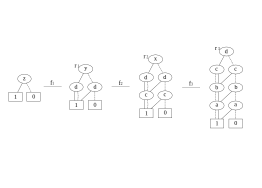
\includegraphics[scale=1.4]{figures/red_steps.pdf}
\caption{Reduction of output of the circuit in Fig. \ref{ChainOrGate} by $f_1,f_2,f_3$.}
\label{red_steps}
\end{figure*}

Consider the circuit shown in Fig. \ref{ChainOrGate} consisting of a
chain of OR gates. Impose RTTO: i.e. {\it lex} term order with
variable ordering as, $z>y>x>d>c>b>a$. The Boolean polynomials for the
circuit are: 
\begin{align}
f_1 = z + y d + y +d;\\ 
f_2 = y + x c + x +c; \\
f_3 = x + b a + b +a;
\end{align}

Under RTTO, the set $G = \{f_1, f_2, f_3\}$ forms a GB. To derive a
canonical representation of the function, we have to reduce the
output $z\xrightarrow{G}_+r$. A classical symbolic algebra
reduction using an explicit representation is carried out as follows: 

\begin{enumerate}
\item { $z \xrightarrow{f_1} y d +y +d$}
\item { $y d +y +d \xrightarrow{f_2} y + xdc + xd + dc + d \xrightarrow{f_2} xdc + xd + xc + x +dc + d + c$}
\item { $xdc + xd + xc + x +dc + d + c \xrightarrow{f_3} xd + xc + x  +
  dcba  + dcb + dca + dc + d + c \xrightarrow{f_3} xc + x + dcba +dcb
  + dca + dc + dba + db + da + d + c \xrightarrow{f_3} x  +dcba +dcb +
  dca + dc + dba + db + da + d + cba + cb + ca + c \xrightarrow{f_3}
  dcba +dcb + dca + dc + dba + db + da + d + cba + cb + ca + c + ba +
  b +a=r$}
\end{enumerate}


% In the first step, $z$ is reduced by $f_1$ just {\it once} as that's the only term. In the
% second step, the result of step one is reduced {\it twice} by $f_2$ as
% the result has two terms containing variable $y$. Similarly,
% {\it four} reductions by $f_3$ are required to 
% reduce the result of step two into an expression containing only
% primary inputs (which cannot be reduced further). 

{\it Observations:} i) Notice that the size of the final remainder 
corresponds to that of the worst case of a Boolean polynomial:
i.e. $r$ contains $2^n - 1\ (=15)$ monomial terms for $n\ (=4)$ variables. ii)
Classical division algorithms reduce the polynomials 1-step at a time,
where only one monomial is canceled in each step. iii) The number of
1-step reductions can increase exponentially as GBR progresses across
the circuit. 

It is clear that any data-structure that {\it explicitly} represents
each monomial will encounter space and time explosion: this includes
the dense-distributive representation of {\sc singular} computer
algebra tool \cite{DGPS}, or the ones used by
\cite{ciesielski:dac2015,rolf:date16}. The $F_4$-style
polynomial reduction of \cite{lv:tcad2013,pruss:tcad} simulates
division on a matrix $M$ representing the problem. However, each column
of $M$ corresponds to a monomial generated in the division process,
therefore \cite{lv:tcad2013,pruss:tcad} also encounter this size
explosion. 

The use of ZDDs can help overcome this explosion. Fig. \ref{red_steps} shows
the same reduction of $z$ by $f_1,f_2,f_3$ using ZDDs (exact
procedure discussed later). The size of the ZDDs after complete reduction by
$f_1,f_2,f_3$ increases linearly in the number of nodes. Subsequently,
the final remainder has $2\cdot n - 1\ (=7)$ nodes (excluding the
terminal 1 and 0 nodes) for $n\ (=4)$ variables. Notice that while
this controls space explosion, the number of paths (monomials) in the
ZDD is still exponential in the number of variables. A classical
division algorithm that cancels only one monomial at a time may still
require an exponential number of iterations. We show how to improve upon
such a situation. 

%\begin{Proposition}
%For the worst case of the Boolean polynomial $F$ with $n$ variables and
%$2^n - 1$ monomials, the ZDD representation of $F$ consists of
%$2\cdot n -1$ nodes in the graph.
%\end{Proposition}
%\debug{somewhere we need to put the objective}

%{\bf ZDD Representation:} %% We show how reduction is performed using
%% ZDDs. 
{\it Problem Setup:} Given a circuit $C$, denote all its {\it nets}
with variables $x_1,\dots,x_n$. Let the total number of gates in the
circuit be $s$; represent each gate of the circuit with a polynomial
$f_i$ in its immediate inputs. Then $F = \{f_1,\dots,f_s\}$ describes
the circuit netlist as a set of Boolean polynomials in
$\Ftwo[x_1,\dots,x_n]$.  

{\it Objective:} Impose RTTO on the polynomial ring, so that the set
$F = \{f_1,\dots,f_s\}$ constitutes a \Grobner basis $G$. For all
primary outputs $z_i \in \{x_1,\dots,x_n\}$, compute
$z_i\xrightarrow{G}_+r_i$ where $r_i$ is the canonical representation
of $z_i$ modulo G, and use it for equivalence checking. The
representation of the polynomials $F$ of $C$, and the computation
$z_i\xrightarrow{G}_+r_i$ is to be performed using ZDDs. 

\subsection{ZDD representation for the polynomials of the circuit}


First, a reverse topological traversal of the circuit is performed to
derive the variable order $x_1 > x_2 > \dots > x_n$ as given in
Prop. \ref{prop:top-order}. The same variable order is imposed on the
ZDDs, i.e. $x_1$ is the variable at the top level in the ZDDs. A
ZDD is created for each variable $x_i$. Using Eqn. (\ref{b2poly})
the gates of the circuit are modeled as the set of Boolean polynomials
$F=\{f_1,\dots,f_s\}$. ZDDs for these polynomials 
%using Eqn. (\ref{eqns:reduce1}) 
are constructed using the $+$ and $\cdot$ binary operations for modulo
2 sum and product of two ZDDs.
%are implemented using {\it ite} operations.
%  really correspond to $\oplus, \wedge$ respectively. 
%
% The operation $lm(f)\over lm(g)$ can be implemented using
%  cube-division in ZDDs.
Conceptually, the modulo 2 sum $(\oplus)$ operation for two ZDDs
$f,g$ can be implemented as $f + g = f_{cs}\cup g_{cs}-f_{cs}\cap g_{cs}$, 
where $f_{cs}$ and $g_{cs}$ represent the cube sets for the
polynomials $f$ and $g$ respectively. For example, let $f = ab + c$
and $g = c + d$ with the corresponding cube sets 
$f_{cs} = \{ab,c\}$ and $g_{cs}=\{c,d\}$, then $f_{cs}\cup g_{cs} = \{ab,c,d\}$
and $f_{cs} \cap g_{cs} = \{c\}$. The set difference $f_{cs} \cup g_{cs} - f_{cs}
\cap g_{cs}$ is the set $\{ab,d\}$ and the corresponding Boolean
polynomial is $ab + d$.  


Experience has shown that such an implementation with the
union operation results in large size of intermediate ZDDs. In order
to avoid this intermediate size explosion, we have implemented the
$f+g\pmod 2$ operation along similar lines as presented in
\cite{polybori:2009}. The algorithm for this operation is shown in
Algorithm \ref{mod2sum}.  

\begin{algorithm}
\caption{Algorithm for performing $f+g\pmod 2$}
\label{mod2sum}
\begin{algorithmic}[1]
{\small
\Procedure{$mod\_2\_sum$}{$f,g$}
\If{$f=0$}
\State \Return $g$
\ElsIf{$g=0$}
\State \Return $f$
\ElsIf{$f=g$}
\State \Return 0
\Else
\State $v_1 = top\_var(f); v_2 = top\_var(g);$
\If{$index(v_1) < index(v_2)$}
\State \Return ${\mathit{ite}}(v_1,then(f),else(f)+g)$
\ElsIf{$index(v_1) > index(v_2)$}
\State \Return ${\mathit{ite}}(v_2,then(g),else(g)+f)$
\Else
\State \Return ${\mathit{ite}}(v_1,then(f) + then(g),else(f)+else(g))$
\EndIf


\EndIf
\EndProcedure
}
\end{algorithmic}
\end{algorithm}

%In the above algorithm, the function $top\_var$ returns the root
%variable for the input ZDD ($f$ or $g$). The function $ite$ is an
%$if$-$then$-$else$ operator used for constructing new ZDDs. The
%algorithm first checks the  simple corner cases in the beginning of
%the algorithm and then depending on the index values of the variables
%(which in our case is RTTO) it recursively constructs  new ZDDs using
%the $ite$ function.  

\begin{Example}
To demonstrate $f+g, f = ab+c, g = c+d$, let the variable ordering be
$a>b>c>d$, i.e. index values for these variables are $0,1,2,3,$
respectively. The condition $index(v_1=a) < index(v_2=c)$ is true. The 
${\mathit{ite}}$ operation places $then(f) = b$ on the solid edge of the root of
the new ZDD and performs $else(f) + g \pmod2$, as shown in 
Fig. \ref{mod2sumfig}. During this recursive call, the last condition
is true  (as $index(v_1=c) = index(v_2=c) = 2$). This time the  ${\mathit{ite}}$
operation performs two recursive calls $then(f) + then(g)$ and
$else(f) + else(g)$, and so on, to finally construct the ZDD for the
Boolean polynomial $ab+d$.

%% The recursive call $then(f) + then(g)$ returns 0 as  
%% both of them are 1 whereas the recursive call $else(f) + else(g)$
%% returns $d$ as $else(f) = 0$ and $else(g) = d$. Therefore $ite$
%% operation creates a ZDD with root $c~(= v_1 = v_2)$ and its
%% 1-$child$ pointing to 0 and 0-$child$ pointing to $d$. Due to the
%% ZDDs' reduction rules, it gets simplified to  just $d$. Therefore,
%% the resultant ZDD of the operation $(ab+c)+(c+d)$ has $a$ as its
%% root, 1-$child$ as $b$, and 0-$child$ as $d$ while representing the
%% boolean polynomial $ab+d$. 
 
\end{Example}

\begin{figure*}[hbt]
\centering
\includegraphics[scale=1]{figures/mod2sumfig_new_1.pdf}
\caption{{$f+g\pmod 2$ using ZDDs}}
\label{mod2sumfig}
\end{figure*}

A similar recursive algorithm is also implemented for $f\cdot g \pmod
2$ operation where the intermediate partial product terms are added
$\pmod{2}$ using the Algorithm \ref{mod2sum}. {\it E.g.,} $f = ab, g =
a+b, f\cdot g = ab + ab = 0$. 


\subsection{GBR $z_i\xrightarrow{G}_+r_i$ under RTTO on ZDDs}


% The variable ordering imposed on the ZDDs is the same as the one
% derived through RTTO. Then every path from the root to terminal {\bf
%   1} represents a monomial, with the 1-edge or solid-edge (resp. 0-edge or dotted-edge) denoting
% the presence (resp. absence) of the variable in the
% monomial. Traversing only the solid edges from the root node of a ZDD to
% terminal {\bf 1} delivers the leading monomial $lm(f)$. The
% child node of the root at the solid edge's end will be referred to as $then$ and the other child as $else$. 

Once the ZDDs for the circuit have been built and stored in $G$, we
need to perform the canonical \Grobner basis reduction $z_i
\xrightarrow{G}_+r_i$ for each output bit $z_i$. The polynomial $r_i$
will be a canonical representation of $z_i$ in terms of primary
inputs. Reduction $f\xrightarrow{g} r$ requires one to obtain the leading
monomials $lm(f),lm(g)$ of $f, g$ (Eqn. \ref{eqns:reduce1}).


\subsubsection{Finding the leading monomials under RTTO on ZDDs}
Recall that RTTO imposes a $lex$ term order on the polynomials using
the variable order $x_1>\dots>x_n$. Moreover, the same variable order
$x_1>\dots>x_n$ is imposed on the ZDDs. Traversing the
then-edges from the root node of a ZDD to terminal {\bf 1}
delivers the leading monomial of that polynomial under RTTO.



\subsubsection{Classical reduction with ZDDs: Cancel one monomial in
  every step} 

The algorithm for conventional reduction procedure using ZDDs is
shown in Algorithm~\ref{singlemon}. The input parameters are the ZDD
of the output bit $z_i$ of the circuit and $poly\_list$ -- a list
containing the ZDDs for the set of polynomials $F =
\{f_1,\dots,f_s\}$ corresponding to the
gates of the circuit. The algorithm is based on the same principles as
the classical division procedure (Algorithm~\ref{algo:mv_reduce}). 
%The variables in the ZDD manager are
%declared in the same order as the RTTO. For our example of
%Figure~\ref{ChainOrGate}, the first variable declared in the ZDD
%manager is $z$, then $f$, and so on. 



%\vspace{-0.2in}

%\vspace{-0.2in}
\begin{algorithm}
\caption{Reduction: Cancel 1 monomial every iteration}
\label{singlemon}
\begin{algorithmic}[1]
{\small
\Procedure{$single\_mon\_red$}{$z_i,poly\_list$}
\For{each $g \in poly\_list$}
\State $lead\_g = leading\_term(g)$
\State $lead\_z_i = leading\_term(z_i)$
\State $quotient = ZDD\_Divide(lead\_z_i,lead\_g)$
\While{$quotient \neq zero$}
\State $prod = quotient \cdot g$
\State $z_i = z_i + prod$
\State $lead\_z_i = leading\_term(z_i)$
\State $quotient = ZDD\_Divide(lead\_z_i,lead\_g)$
\EndWhile
\EndFor
\State \Return $z_i$
\EndProcedure
}
\end{algorithmic}
\end{algorithm}

The procedure $leading\_term(g)$ returns the leading term of 
the ZDD representation of polynomial $g$. 
%The procedure starts at the root node and follows the THEN path until
%it reaches the terminal node 1. The cube of the variables, whose
%corresponding nodes are encountered on this path, gives us the
%leading term of the polynomial. 
If $g$ divides $f$, then the procedure $ZDD\_Divide(f,g)$ (performs cube division) returns the quotient of the
division,  else it returns zero. Line 8 computes $z_i = z_i +
{lt(z_i) \over lt(g)}\cdot g$. The polynomial $z_i$ is completely reduced
$w.r.t.$ the polynomial $g$ in the while loop. 
% The $\cdot$ operator
% computes the product of two ZDDs and the + operator is a modulo 2
% sum: $f + g = f \cup g - f \cap g$. 

\subsubsection{Improved Reduction: Cancel multiple monomials in 1 step}
Next, we will show how $z_i$ can be reduced by a polynomial $g$ {in one step}. In the 
example of Figs. \ref{ChainOrGate} and \ref{red_steps}, the primary output
$z$ is reduced by $f_1$ to get $r_1$. The next  step  
is to reduce $r_1$ by $f_2$ to get $r_2$. To demonstrate our
approach we will show how the reduction of $r_1$ by $f_2$ can be
achieved in one step. There are two monomials in $r_1$ that contain
$y$, namely $yd,y$. Both can be canceled by $lt(f_2) = y$ in one step,
eliminating the need of the while loop in Algorithm~\ref{singlemon}.    

The polynomial $r_1 = yd + y + d$ can be written as $y\cdot(d+1) +
d$. If we perform 1-step reduction of $r_1$ by $f_2$ we get 
the {\it quotient} $d+1$. This quotient is visible as the polynomial
represented by the $then$-node of $r_1$ (Fig. \ref{f2}). So the
reduction can be performed by multiplying $d + 1$ with $f_2$ and
subtracting (adding) this  product to $r_1$ $\pmod{2}$.
% \vspace{-0.1in}
%{\small
\begin{align}
& r_1\xrightarrow{f_2}_+ r_2\\
&= (yd + y + d) + (d + 1)\cdot(y + xc + x + c) \pmod{2}\\
&= 2\cdot(yd + y) + d + (d+1)\cdot(xc + x + c) \pmod{2}\label{eqn:cancelmon}\\
&= \underbrace{d}_{else(r_1)} + \underbrace{(d+1)}_{then(r_1)}\cdot\underbrace{(xc + x + c)}_{else(f_2)}  \pmod{2}
\label{eqn:subexp}
\end{align}
%\vspace{-0.1in}
%Use the follwing notation
%\begin{align*}
%& \text{$head(R_1)$ = 1-branch (THEN) of top-most node of $R_1$} = d + 1,\\
%& \text{$tail(R_1)$ = 0-branch (ELSE) of top-most node of $R_1$} = d,\\
%& \text{$head(P)$ = 1-branch of top-most node of $P$} = f,\\
%& \text{$tail(P)$ = 0-branch of top-most node of $P$} = ec + e + c.
%\end{align*}
%}
As shown in Fig. \ref{f2}, $else(r_1)=d, then(r_1)=d+1$ and
$else(f_2)=xc+x+c$. Moreover, $2\cdot(yd + y) = 0
\pmod{2}$. Therefore, in order to reduce number of operations incurred
in the division process, we directly use the last step as a formula
for reduction:   
%\vspace{-0.05in}
%{\small
\begin{align}
\label{eqn:onestep}
r_1 \xrightarrow{f_2}_+ r_2 %&= d + (d+1)\cdot(xc + x + c) \\
&= else(r_1) + then(r_1)\cdot else(f_2)
\end{align}
% }%

\begin{figure}[hbt]
\centering
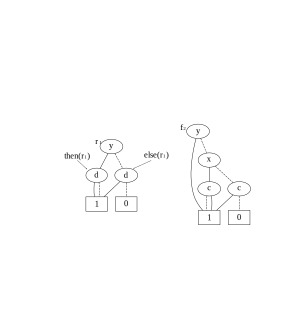
\includegraphics[scale=1]{figures/r1_f2.pdf}
\caption{ZDDs for polynomial $r_1$ and $f_2$.}
\label{f2}
\end{figure}

%In order for the above equation to be correct in general, 
More generally, to perform the division $r_i \xrightarrow{f_j}_+ r_j$, 
we need to ensure that if $f_j$ divides $r_i$, then the variable
(index) associated with the top-most nodes of  their respective ZDDs
are the same. This can be ensured by populating
$poly\_list=\{f_1,\dots,f_s\}$ in a certain order.
%This also results in a significant improvement in
%Algorithm \ref{singlemon} by simplifying the search for the divisors
%$g\in poly\_list$ and is described in the next paragraphs and Example \ref{exm:pi_rtto}.

Due to RTTO, each polynomial $f_j \in F$ is of the form $f_j = x_j +
\text{tail}(f_j)$, where each variable in $\text{tail}(f_j)$
is ordered as being less than $x_j$ (Prop. \ref{prop:top-order}). Due to this order,
the ZDD representation of the polynomials is of the type $f_1= x_1 +
else(f_1), \dots, f_s= x_s + else(f_s)$, where the variables $x_1,\dots,x_s$ are the 
top-most nodes in their respective ZDDs with variable order $x_1 >
\cdots > x_s > \cdots > x_n$. Note that the variables
$\{x_{s+1},\dots,x_{n}\}$ are the primary inputs, and they are not the output
of any logic gate. {\it We ensure that primary inputs appear last in RTTO.}
Then we store elements in $poly\_list$ according to the order
$f_1 > f_2 > \dots > f_s$; i.e. $poly\_list[1] = f_1,
\dots,poly\_list[s] = f_s$. 

Considering Algorithm \ref{singlemon}, suppose
that we first reduce $z_i$ by $poly\_list[1]=f_1$, which results in
variable $x_1$ being replaced by $tail(f_1)$ in $z_i$. The
variable $x_1$ cannot appear  again in $z_i$ at any further reduction
step as $x_1$ is not in the support of  polynomials
$poly\_list[2],\dots,poly\_list[s]$. Further in the reduction process,
let us assume that we have reduced $z_i$ by 
$f_1,f_2,\dots,f_{j-1}$. At this stage the intermediate remainder
$z_i$ will not contain any of the variables $x_1,x_2,\dots,x_{j-1}$ as
they have been canceled by the leading terms of
$f_1,f_2,\dots,f_{j-1}$. The next variable in RTTO is $x_j$.
%
%The variables next to $x_{j-1}$ in RTTO is $x_j$ 
%Therefore, the top-most
%node in the ZDD of $z_i$ can be any one of the variables
%$x_j,\dots,x_n$. It need to be just $x_j$ as all variables 
%may not be in the logical cone of $z_i$. 
To cancel terms in $z_i$ containing variable $x_j$, we need to search
for the divisor polynomial $f_j = x_j + tail(f_j)$. 
%
There can be two possibilities for $z_i$: 
\begin{enumerate} 
\item If terms in $z_i$ contain
$x_j$, then the top variable of the ZDD of $z_i$ will be $x_j$. In
  that case, as the top variable of the ZDD of $f_j$ is also $x_j$,
  $f_j$ can divide $z_i$.
\item If $z_i$ does not contain terms in $x_j$, then the top variable
  of the ZDD of $z_i$ will not be $x_j$. In that case, $f_j$ (with
  top variable $x_j$) cannot divide $z_i$. 
\end{enumerate}
Therefore, the divisibility of $z_i$ by  the current entry in
$poly\_list[j] = f_j$ can be checked just by comparing the indices of
the top nodes of the ZDDs of $z_i$ and $f_j$. If the indices 
are equal, then $f_j$ divides $z_i$. Otherwise, $f_j$ does not divide
$z_i$. 
% In terms of the topology of the circuit, the latter case
% implies that the gate corresponding to polynomial $f_j$ is not in the
% logical cone of $z_i$. 
% As a result, imposition of RTTO on the ZDDs and on $poly\_list$ simplifies the check
% for divisors: {\it if indices of top-most nodes of ZDDs of $z_i$ and
%  $f_j$ are equal, then $lm(f_j)$ divides $lm(z_i)$.} 
This allows to 
replace the cube division (Line 5, Algorithm \ref{singlemon}) by an
equality check of top indices of ZDDs.

% \begin{Example}
% \label{exm:pi_rtto}
% Consider the step 2 of division corresponding to
%  Fig. \ref{ChainOrGate}, where the polynomial $r_1 = yd +y+d$ needs to
%  be reduced by $f_2$. RTTO need not differentiate between the
% relative ordering of the nets $y, d$ for Prop. \ref{prop:top-order} to
% be valid; as both $y, d$ are at the same (reverse) topological
% level. However, we ensure that the primary inputs always appear last
% in the order. The ZDDs for $r_1$ and $f_2$ are shown in
% Fig. \ref{f2}, where RTTO is lex with $y > x > d > c > b> a$.  As
% $index(top\_var(f_2)) = index(top\_var(r_1))$,  $lm(f_2) ~|~ \textcolor{red}{lm(r_1)}$.
% If variable $d$ were placed earlier in the order than $y$, then the
% top variables of $f_2, r_1$ 
% would have been different and we would have had to extract
% $lm(r_1),lm(f_2)$ and performed cube division
% ${lm(r_1)}\over{lm(f_2)}$ to check if $lm(f_2) ~|~ lm(r_1)$. 
% \end{Example}


%% While iterating over the polynomials $g \in poly\_list$ if a
%% certain polynomial does not divide the leading term of $z_i$, it 
%%  will imply the polynomial is not in the logical cone of $z_i$.   

Therefore, unlike in Algorithm~\ref{singlemon}, where we need to
obtain the leading monomials and compute the quotient
$lead\_z_i/lead\_g$, now we only need to determine if
$lead\_g$ can divide $z_i$ at all (in which case the quotient is
$then(z_i)$). This can be accomplished by just comparing the indices
of top-most nodes of $z_i$ and $g$. 

\par It can now be shown that Eqn. (\ref{eqn:onestep})
holds throughout the GB-reduction under RTTO. To perform the operation
$r_i\xrightarrow{f_j}_+ r_j$, we consider their ZDDs constructed
using RTTO. Based on the above discussion, the top variables of the
ZDDs of $r_i$ and $f_j$ are the same and equal to $x_j$. Also, let $q$
denote the quotient of division of $r_i$ by $f_j$. The operation $r_i
\xrightarrow{f_j}_+ r_j$, is carried out as follows, 
\begin{align*}
r_j &= r_i + q\cdot f_j  
\end{align*}
As $x_j$ is the top variable of $r_i$ and $f_j$, they can be written
as $r_i = x_j\cdot then(r_i) + else(r_i)$ and $f_j = x_j + else(f_j)$,
respectively. Also notice that $q = then(r_i)$, because $f_j$ (with
leading term $x_j$) can only divide the $x_j\cdot then(r_i)$ component
of $r_i$. 
\begin{align*}
r_j &= x_j\cdot then(r_i) + else(r_i) + q\cdot(x_j + else(f_j)) \\
 &= x_j\cdot then(r_i) + else(r_i) + then(r_i)\cdot(x_j + else(f_j)) \\
 &= 2\cdot x_j\cdot then(r_i) + else(r_i) + then(r_i)\cdot else(f_j) \\
 &= else(r_i) + then(r_i)\cdot else(f_j)
\end{align*}
\par The last expression is the same as in
Eqn. (\ref{eqn:onestep}). So the reduction process effectively
involves just two operations, a modulo 2 sum and a product. {\it This
  has the effect of canceling all the terms in $r_i$ that can be
  canceled by $lt(f_j)$,  implicitly canceling multiple monomials in
  one step}.  This is made possible only due to the properties that
RTTO imposes on the structure of ZDDs. 

The algorithm for implicit cancellation of multiple monomials in
GB-reduction is shown in Algorithm~\ref{multimon}, where the notations,
$z_i$ and $poly\_list$, are the same as in Algorithm
\ref{singlemon}. This algorithm significantly
reduces the number of iterations, which now exactly equals the size of
$poly\_list$. For the example of Fig. \ref{ChainOrGate}, the number of
iterations is 3 using Algorithm~\ref{multimon}, whereas 7 iterations
are required using Algorithm \ref{singlemon}.


\begin{algorithm}
\caption{Reduction under RTTO: Cancel multiple monomials}
\label{multimon}
\begin{algorithmic}[1]
{\small
\Procedure{$multi\_mon\_red$}{$z_i,poly\_list$}
\For{each $g \in poly\_list$}
%\State $G_i = POLY\_LIST[i]$
%\State $index_{G_i} = G_i \rightarrow index$
%\State $index_F = F \rightarrow index$

\If{ $index(g) == index(z_i)$} 
%\State $p_1 = then(f)$
%\State $p_2$ = else(f)
%\State tail = else($g_i$)
%\State prod = $p_1$ $ \cdot$  tail
\State $z_i = else(z_i) + then(z_i)\cdot else(g)$
\EndIf

\EndFor
\State \Return $z_i$
\EndProcedure
}
\end{algorithmic}
\end{algorithm}


   

% To contrast our approach against PolyBori \cite{polybori:2009}:
% PolyBori is a general purpose symbolic computing engine for Boolean
% polynomials, whereas our approach (Algorithm
% \ref{multimon}) is specific only to RTTO; it would give an incorrect
% result of reduction for non-RTTO based term orders. However, our
% approach exploits the fact that due to RTTO, the subexpressions
% required in the division process are readily
% available as the $then$- and $else$-children of the top nodes of the
% ZDD (Eqn. (\ref{eqn:subexp})). Moreover, an implementation using
% PolyBori may also generate intermediate monomials that eventually add
% up to 0 $\pmod 2$  ($e.g.$ as in Eqn. (\ref{eqn:cancelmon})). Whereas
% our approach reduces the size of intermediate computations, and incurs
% less computation time, by not generating the duplicate monomials. 


We have implemented the above GBR procedures using the CUDD 
package~\cite{cudd}. The circuit under verification is analyzed, RTTO based
variable order is imposed on the ZDDs, and the Boolean polynomials of
the circuit are represented as unate cube sets on ZDDs. 
The polynomials corresponding to the gates of circuit,
$G=\{f_1,\dots,f_s\}$, are inserted in $poly\_list$ according to the
variable order $x_1 > \dots > x_i > \dots > x_n$, where $f_i = x_i +
else(f_i)$. % (this is due to Prop. \ref{prop:top-order}). 
To perform GBR $z_i\xrightarrow{G}_+ r_i$,
Algorithm \ref{multimon} is invoked and $r_i$ used for  equivalence checking. 
%The division algorithm in {\sc
%  polybori} \cite{polybori} is conceptually similar to that of
%Algorithm 1, whereas Algorithm 2 is our main contribution.

%\documentclass{article}
%\documentclass[10pt,twocolumn]{IEEEtran}
%\usepackage[a4paper, margin=1in]{geometry}%lmargin=1in, rmargin=1in, tmargin=1in, bmargin=1in]{geometry}
%\usepackage{algorithm}
%\usepackage{algpseudocode}
%\usepackage{svg}
%\usepackage{xcolor}
%\usepackage{multirow}
%\usepackage{booktabs}
%\bibliographystyle{plain}
%\usepackage{float}
%\usepackage{boldline}
%\usepackage{pbox}
%\usepackage{tabularx}
%\usepackage{graphicx}
%\usepackage{amsmath}
%\usepackage{amsfonts}

%\begin{document}

\section{EXPERIMENTAL RESULTS}
\label{sec:exp}
\iffalse
%\iffalse
This section presents the results of reducing modulo multiplier
circuits used in cryptography using our implementation. The
experiments are performed on a 3.5GHz Intel 
Core\textsuperscript{TM} i7-4770K Quad-Core CPU with 32 GB of RAM. There are
two architectures that implement these multipliers, namely Mastrovito
and Montgomery. 
Mastrovito multipliers compute $Z = A\times B \pmod{
  P}$
%take $\{A,B\} =
%\{a_0,a_1,\dots,a_{k-1},b_0,b_1,\dots,b_{k-1}\}$ as $k$-bit inputs and
%produce $Z = \{z_0,z_1,\dots,z_{k-1}\}$ as $k$-bit output. The multiplier
%performs $Z = A \times B \pmod{P}$, 
where $P$ is a given primitive polynomial for the datapath size
$k$. 
%The procedure 
%involves computing the product $S=A\times B$ using an array multiplier
%and then reducing it $\pmod{P}$ to obtain $Z$. We perform experiments
%on \textit{flattened} netlists of these circuits.  
Montgomery multipliers perform fast modular multiplication without
explicitly performing the reduction $\pmod{P}$. 
%They are more
%efficient than the Mastrovito multipliers when several modulo
%multiplications are required as in the case of exponentiation in
%cryptosystems. 
Fig.~\ref{montfig} shows the structure of a Montgomery
multiplier. Each MR block computes $A\cdot B\cdot R^{-1}$, where $R$
is selected as a power of a base ($\alpha^{k}$). We denote the leftmost
two blocks as Block A (upper) and B (lower), the middle block as Block
C and the output block as Block D. We have presented results for GBR
on both \textit{flattened} and \textit{hierarchical} netlists of these
multipliers. 

\begin{figure}[H]
  \centering
  %\def\svgwidth{340pt}
  \includegraphics[scale=0.34]{new_mmcircuit}
  \caption{Montgomery multiplication}
  \label{montfig}
  \end{figure}

 
Table~\ref{masmm} provides the statistics on the time, ZBDD size, and
savings in the number of monomial cancellations achieved by our
approach as compared to classical symbolic algebra methods, for
Mastrovito multiplier circuits. The time reported is the total time
required to perform the reduction, $z_i \xrightarrow{G}_+ r_i$, for
all $i = 0,\dots,k-1$. The columns 
\textit{F4}, \textit{PB}, and \textit{ZR} represent the time taken in
seconds by F4 style reduction, PolyBori (version 0.8.3) and our
implementation respectively. \textit{MN} represents the maximum size
of any ZBDD encountered during reduction of any output-bit, while
\textit{MR} represents the maximum size of the ZBDD among all final
remainders $r_i$. \textit{CS} represents the
number of iterations saved during reduction due to our implicit
method. PolyBori throws a segmentation fault for the multiplier with
$k = 571$ which is depicted as \textit{CR} in the table. Our approach
is orders of magnitude faster than both \textit{F4} and \textit{PB}. 

Table~\ref{montmm} provides the same statistics for \textit{flattened}
Montgomery multipliers. The data for \textit{MN} and \textit{CS}
columns in  case of  $k=571$ could not be procured as both these
operations require traversal along ZBDDs (using the procedure {\tt
  Cudd\_zddDagSize()} and {\tt Cudd\_zddNextPath}). As there is a huge
number of large-sized intermediate ZBDDs produced during this
reduction, traversing along each path of every ZBDD is
infeasible. Also, the reduction times for $k=283$ is inordinate when
compared to other datapath sizes, which is purely due to  the
structure of the circuit.  


%The reduction times for $k=283$ is inrodindate when compared to other datapath sizes, which is purely due to the structure of this circuit.

%Table~\ref{montblockmm} and~\ref{montblockstats} depicts the comparison of time, ZBDD size, and monomial savings across \textit{Montgomery} Flat multiplier circuits with different field sizes. \textit{F4}(F4 style abstraction)*reference to Tim's paper*, \textit{PB}(PolyBori), and \textit{ZR}(ZBDD Reductions) represents the time in seconds for the respective implementations. \textit{MN}(Max Nodes) represents the maximum number of ZBDD size encountered, while \textit{MR}(Max Remainder) represent the maximum size for any remainder after the reductions. \textit{CS}(Cancellation Savings) signifies the total amount of monomial savings with our implementation.

%Table~\ref{montblockmm} depicts the comparison of ZBDD max size, remainders, and monomial savings across \textit{Montgomery} Block multiplier circuits with different block sizes, given different field sizes. For a given Block and field size, \textit{MN}(Max Nodes) represents the maximum number of ZBDD size encountered, while \textit{MR}(Max Remainder) represents the maximum size for any remainder while doing reductions with our implementation. \textit{CS}(cancellation savings) signifies the total amount of monomial savings with our implementation.

Table \ref{montblockmm} present the
statistics for hierarchical Montgomery multipliers for the blocks A,
B, C, and D. The experiment first reduces the outputs of a block
modulo the gates of that block, and then reduces the primary outputs
modulo these four sets of remainders (ZBDDs), thus exploiting the
hierarchy of these circuits. Table~\ref{montblockmm} shows the time
for reduction of each block and the time for reducing the primary
outputs across the four levels. The  time for reducing the primary
outputs across  levels in case of F4 implementation is $<$1 second,
and is not explicitly mentioned in the table. The row labeled
\textit{Total} presents the sum of time of reduction across levels and
the maximum reduction time for each block (as the reductions for the
four levels are independent of each other and are done in
parallel). The datapath sizes of these circuits correspond to
NIST-specification in cryptography with $k = 163,\dots,571$ bits.

%\par The reduction time presented in this section is obtained by reducing each output bit sequentially. These runtimes can be further improved by running these reductions in parallel.

%% The reduction times for small integer arithmetic array multipliers are
%% presented in Table \ref{intmm}. There is an 8x increase in time when
%% moving from $n-1$ datapath size to $n$-bits, which is an exponential
%% increase. Performing detailed analysis of a 7x7 multiplier reveals
%% that, when reducing the $z_{13}$ bit (MSB) and $z_{12}$ bit of this
%% circuit, the maximum number of monomials encountered are 429,889 and
%% 897,955. Of these, 269,120 monomials are {\it common to both output
%%   bits}. This implies that integer multipliers require a word-level
%% decision procedure, as given in \cite{ciesielski:dac2015}
%% \cite{rolf:date16}, that account for the cancellation of these
%% monomials across multiple bits in one word-level expression. Our
%% results show that bit-level techniques cannot efficiently verify
%% integer arithmetic circuits, but are very efficient for finite-field
%% arithmetic circuits.    
%\fi


%\iffalse
%%%%%%%%%%%%%%%% Mas Multipliers %%%%%%%%%%%%%%%%%%%
\iffalse
\begin{table}[H]
\centering
%\caption{Mastrovito Multipliers (Time in seconds, \# of nodes, \# of redundant monomials in $k$)  (K = $10^3$, M = $10^6$)}
\caption{Mastrovito Multipliers (Time in seconds)  TO = 3 days, (P):Parallelization, (WP):Without Parallelization}
\label{masmm}
\begin{tabular}{| c | c | c | c | c | c | c |} \hline
%\multirow{2}{*}{\textbf{Input}} & \multirow{2}{*}{\textbf{Abstraction}} & \multicolumn{3}{ c |}{\textbf{ZBDD reduction(ZR)}}  &  \multirow{2}{*}{\textbf{ZR improved}}\\ \cline{3-5}
% & &Building ZBDDs&Reduction&Total&\\ \hline
\textbf{Datapath(k)}&\textbf{\# of Gates} & \textbf{F4} &\textbf{\#T}&\textbf{CX(P)} & \textbf{PB(WP)} & \textbf{ZR(WP)}\\ \hline
163 &153K& 1,443 &30& 110 &70& 9  \\ \hline 
233 &167K& 1,913 &30&169 &105& 9 \\ \hline
283 &399K& 11,116 &30&496&316& 37 \\ \hline
409 &508K& 17,848 &30& 909& 596&39 \\ \hline
571 &1.6M& 192,032 &10&4,245& CR&566 \\ \hline 


\end{tabular}
\end{table}
\fi

%%%%%%%%%%%%%%%%%%%%%%%%%%%%%%%%%%%%%%%%%
%%%%%%%%%%%%%%%% Mont Multipliers %%%%%%%%%%%%%%%%%%
\iffalse
\begin{table}[H]
\centering
%\caption{Montgomery Flat Multipliers (Time in seconds) (K = $10^3$, M = $10^6$, B = $10^9$, No. of threads = T)}
\caption{Montgomery Multipliers (Time in seconds)  TO = 3 days, (P):Parallelization, (WP):Without Parallelization}
\label{montmm}
\begin{tabular}{| c | c | c | c | c | c | c |} \hline
%\multirow{2}{*}{\textbf{Input Bit-width}} & \multirow{2}{*}{\textbf{Abstraction}} & \multicolumn{3}{ c |}{\textbf{ZBDD reduction(ZR)}}  &  \multirow{2}{*}{\textbf{ZR improved}} \\ \cline{3-5}
% & &Building ZBDDs&Reduction&Total& \\ \hline
\textbf{Datapath(k)}&\textbf{\# of Gates} & \textbf{F4} & \textbf{\#T} &\textbf{CX(P)}& \textbf{PB(P)}  &\textbf{ZR(P)} \\ \hline
163 & 184K&6,897 & 20&1,142&5,590&6,224 \\ \hline 
233 & 329K&63,805 &10 &316& 578&468\\ \hline
283 & 488K&TO &10&15,055  &108,168& 129,904 \\ \hline
409 & 1.0M&TO & 3&2,609 &9,350&8,959\\ \hline
571 & 1.97M&TO & 3 &estimated 4days (TO) &CR&43,813 \\ \hline 

\end{tabular}
\end{table}
\fi
%%%%%%%%%%%%%%%%%%%%%%%%%%%%%%%%%%%%%%%%%
\fi

This section presents the results of using our implementation (Algorithm~\ref{multimon}) for reducing
circuits used in cryptography. We compare our results against F4-style reduction~\cite{pruss:tcad}, 
parallelized approach for performing reductions on Galois field multipliers~\cite{cunxi:aspdac17}, 
and PolyBori~\cite{polybori:2009} that uses the conventional reduction procedure on top of ZBDDs. 
The experiments are performed on a 3.5GHz Intel 
Core\textsuperscript{TM} i7-4770K Quad-Core CPU with 32 GB of RAM. 
% Modular multiplication is an important computation used in cryptography. 
% We have performed experiments with two architectures for this multiplication, namely Mastrovito and Montgomery. 

\subsection{Mastrovito Multipliers}

Modular multiplication is an important computation used in cryptography. 
A Mastrovito multiplier architecture can be employed for performing this computation.
Mastrovito multipliers compute $Z = A\times B \pmod{
  P}$ where $P$ is a given primitive polynomial for the datapath size
$k$. 

The product $A \times B$ is computed using an array multiplier architecture, and then the result is reduced modulo $P$.
The following example demonstrates the Mastrovito multiplier computation~\cite{lv:tcad2013}.
%take $\{A,B\} =
%\{a_0,a_1,\dots,a_{k-1},b_0,b_1,\dots,b_{k-1}\}$ as $k$-bit inputs and
%produce $Z = \{z_0,z_1,\dots,z_{k-1}\}$ as $k$-bit output. The multiplier
%performs $Z = A \times B \pmod{P}$, 

%The procedure 
%involves computing the product $S=A\times B$ using an array multiplier
%and then reducing it $\pmod{P}$ to obtain $Z$. We perform experiments
%on \textit{flattened} netlists of these circuits.  

\begin{Example}
\label{exp1}
{\it 
Consider the field $\mathbb{F}_{2^4}$. Let the inputs be:
$A=a_0+a_1\cdot \alpha+a_2\cdot \alpha^2+a_3\cdot \alpha^3$ and
$B=b_0+b_1\cdot \alpha+b_2\cdot \alpha^2+b_3\cdot \alpha^3$, and 
 the irreducible polynomial be $P(x)=x^4+x^3+1$. 
 % We have to perform the multiplication $Z =A\times B \pmod{ P(x) }$. 
 The coefficients of $A = \{a_0, \dots, a_3\}, B = \{b_0, \dots, b_3\}$ are in
$\mathbb{F}_2 = \{0, 1\}$. First, we perform the multiplication as:

%\vspace{-0.2in}

\vspace{0.05in}

{\small
{\begin{tabular}{c c c c c c c c}
%\vspace{-0.2in}
  &   &   & $a_3$ & $a_2$ & $a_1$ & $a_0$  \\ 
 $\times$&   &   & $b_3$ & $b_2$ & $b_1$ & $b_0$  \\ 
 \hline
 &   &   & $a_3\cdot b_0$ & $a_2 \cdot b_0$ & $a_1\cdot b_0$ & $a_0\cdot b_0$ \\
 &  & $a_3\cdot b_1$ & $a_2\cdot b_1$ & $a_1 \cdot b_1$ & $a_0\cdot b_1$ &   \\
 & $a_3\cdot b_2$ & $a_2\cdot b_2$ & $a_1\cdot b_2$ & $a_0\cdot b_2$ &  &   \\
 $a_3\cdot b_3$ & $a_2\cdot b_3$ & $a_1\cdot b_3$ & $a_0\cdot b_3$ &  &  &   \\
 \hline
 $s_6$& $s_5$  & $s_4$  & $s_3$ & $s_2$  & $s_1$   & $s_0$ 
% \vspace{-0.2in}
\end{tabular}}
}

\vspace{0.05in}

The result $Sum = s_0+s_1\cdot \alpha + s_2\cdot \alpha^2 + s_3\cdot
\alpha^3 + s_4\cdot \alpha^4 + s_5\cdot \alpha^5 + s_6\cdot \alpha^6$,
where, $s_0  =  a_0\cdot b_0, ~~s_1  =  a_0\cdot b_1 + a_1\cdot b_0,
~~s_2 = a_0\cdot b_2 + a_1\cdot b_1 + a_2\cdot b_0$, and so on. Here
the multiply ``$\cdot$'' and add ``$+$'' operations are performed
modulo 2, and hence implemented in a circuit using AND and XOR
gates. As the coefficients are always reduced modulo $p =
2$, there are no carry-chains
in the design. Next, the result is reduced modulo the primitive
polynomial $P(x) = x^4 + x^3 + 1$, as:
% where the final output of the circuit is denoted by $G(x)  = g_3x^3
% + g_2x^2 +g_1x + g_0$.  

\vspace{0.05in}

{\small
{\begin{tabular}{|c c c c | l }
  $s_3$   &$s_2$    &$s_1$   &$s_0$   &   \\
 \hline
 $s_4$    &$0$    &$0$   &$s_4$   &$s_4\cdot \alpha^4 \pmod{P(\alpha)} = s_4 \cdot (\alpha^3 + 1)$\\
 $s_5$    &$0$    &$s_5$   &$s_5$     &$s_5\cdot \alpha^5 \pmod{P(\alpha)} = s_5\cdot (\alpha^3+ \alpha + 1)$\\
 $s_6$    &$s_6$    &$s_6$   &$s_6$     &$s_6\cdot \alpha^6 \pmod{ P(\alpha)} = s_6\cdot( \alpha^3 + \alpha^2 + \alpha + 1)$\\
 \hline
 $z_3$    &$z_2$    &$z_1$   &$z_0$   &
 \end{tabular}\par}
}

\vspace{0.05in}

The final output of the circuit is: $Z = z_0 + z_1 \alpha + z_2
\alpha^2 + z_3 \alpha^3$; where  $z_0=s_0+s_4+s_5+s_6; ~~z_1=s_1+s_5+s_6;
~~z_2=s_2+s_6; ~~z_3=s_3+s_4+s_5+s_6$. 
}
\end{Example}

\par Table~\ref{masmmsyn} provides the results for the reductions $z_i \xrightarrow{G}_+ r_i$ for Mastrovito multipliers for each output bit $z_i$.
The benchmarks are taken from~\cite{lv:tcad2013} which are optimized using ABC~\cite{ABCtool} with the same commands and library as mentioned in~\cite{cunxi:aspdac17}. Algorithm~\ref{multimon} reduces each output bit independent of other bits. Therefore, we have presented the results obtained by running our reduction algorithm both parallely and sequentially for each output bit. Similarly, the results for implementation in PolyBori are also presented for both cases. The maximum number of parallel processes is decided by the memory usage of each process ($i.e.$ reducing one bit) for our implementation and the total available memory. The larger benchmarks are run with fewer parallel processes as they consume more memory.
% As ZBDDs are more complex data structures compared to those used in~\cite{cunxi:aspdac17}, the upper limit of memory usage for each bit is set by our implementation. For instance, an individual process in the reduction of 283-bit multiplier can take upto $\sim 3\%$ of available memory as compared to $\sim 6\%$ in the case of 409-bit mulitplier. Therefore, we run the all the implementations with 20 parallel processes for 283-bit multiplier but only with 10 for 409-bit multiplier. 
\par In the table, the column \#T represents the number of parallel processes. (S) and (P) refer to the cases when the experiments are run sequentially and parallely for the output bits $z_i$, respectively. 

%%%%%%%%%%%%% Syn Mas Multipliers %%%%%%%%%%%%%%%%%%%
%\iffalse
\begin{table}[H]
\centering
%\caption{Synthesized Mastrovito Multipliers (Time in seconds, \# of nodes, \# of redundant monomials in $k$)  (K = $10^3$, M = $10^6$)}
\caption{Mastrovito Multipliers (Time in seconds);  k = Datapath Size, \#Gates = No. of gates, \#T = No. of threads, Time-Out = 30 hrs, (P): Parallel Execution, (S): Sequential Execution, K = $10^3$, M = $10^6$, PB: PolyBori, ZR: Algorithm~\ref{multimon}}
\label{masmmsyn}
\begin{tabular}{| c | c | c | c | c | c | c | c | c |} \hline
%\multirow{2}{*}{\textbf{Input}} & \multirow{2}{*}{\textbf{Abstraction}} & \multicolumn{3}{ c |}{\textbf{ZBDD reduction(ZR)}}  &  \multirow{2}{*}{\textbf{ZR improved}}\\ \cline{3-5}
% & &Building ZBDDs&Reduction&Total&\\ \hline
\multirow{2}{*}{\textbf{k}}&\multirow{2}{*}{\textbf{\#Gates}}&\multirow{2}{*}{\textbf{F4~\cite{pruss:tcad}}}& \multirow{2}{*}{\textbf{\#T}}&\multirow{2}{*}{\textbf{~\cite{cunxi:aspdac17}(P)}}& \multicolumn{2}{ c |}{\textbf{PB}}&\multicolumn{2}{ c |}{\textbf{ZR}}\\ \cline{6-9}
&&&&&\textbf{(P)}&\textbf{(S)}&\textbf{(P)}&\textbf{(S)} \\ \hline
64 &11.5K&1.3&20& 3.70&3.60& 2.21&0.73 &\textbf{0.27}\\ \hline 
% 96 &25.6K&&20& 11.66&10.25&6.92 &2.04 &\textbf{0.66}\\ \hline 
128 &46K&9.89&20&27.54 &23.99&16.76& 5.08 &\textbf{1.63}\\ \hline 
163 &73.5K&32.61&20& 55.96&48.67&33.72&  11.41&\textbf{3.11}\\ \hline 
233 &122K&86.30& 20&127.61&112.96 &77.23& 21.77&\textbf{3.63}\\ \hline
283 &193K&274.68& 20&253.05&227.77&157.45& 49.89&\textbf{11.41}\\ \hline
409 &386K&2,528.48& 10&716.80 &659.64&426.92& 163.52&\textbf{17.68}\\ \hline
571* &1.6M & TO &3 & 5,331&CR&CR&2,126.65& \textbf{566.39}\\ \hline
\end{tabular}
\end{table}
%\fi

%%%%%%%%%%%%%%%%%%%%%%%%%%%%%%%%%%%%%%%%%
\par The 571-bit multiplier could not be synthesized and mapped with the given memory. Therefore, we have provided results for a structured (but not optimized) 571-bit multiplier benchmark. Our implementation outperforms the explicit approaches of~\cite{pruss:tcad} and~\cite{cunxi:aspdac17} for Mastrovito multipliers. For the 571-bit multiplier, the implementation of~\cite{pruss:tcad} does not finish for the given time period of 30 hours and the PolyBori implementation crashes (CR).

\par An interesting point to note in the Table~\ref{masmmsyn} is that our implementation takes less time when we are running it sequentially. There is a certain overhead involved when we declare variables and build ZBDDs for each gate of the circuit. In the case of Mastrovito multipliers benchmarks, this overhead is substantially greater than the reduction time for each output bit. Therefore, when we run these benchmarks parallely this overhead time hampers the overall run time. 
% For example, for the 64-bit multiplier the overhead is 22.09 ms (when running it sequentially), whereas the reduction time for most of the bits is $\sim 0.30$ ms. The sequential reduction time with these values is $22.09 + 64 (0.3) = 41.29$ ms. On the other hand, with 20 processes this time is approximately $(64/20)(22.09 + 0.3) = 71.65$ ms. 
% There are other factors involved too, $e.g.$ CUDD package maintains an internal cache that helps avoid duplicate computations. When performing reduction sequentially the operations involving fanouts can be stored in the cache and used during the reduction of different output bits. 
 

\subsection{Montgomery Multipliers}
Exponentiation (repeated multiplication) is often required in cryptosystems.  
For such applications, Montgomery architecture \cite{acar:1998} \cite{wu:2002}
% \cite{Barrett:1987} 
\cite{Knezevic:2008} are considered more efficient than Mastrovito multipliers
as they do not require explicit reduction modulo $P$ after each step.
% Montgomery multipliers perform fast modular multiplication without
% explicitly performing the reduction $\pmod{P}$. 
%They are more
%efficient than the Mastrovito multipliers when several modulo
%multiplications are required as in the case of exponentiation in
%cryptosystems. 
Fig.~\ref{montfig} shows the structure of a Montgomery
multiplier. Each MR block computes $A\cdot B\cdot R^{-1}$, where $R$
is selected as a power of a base ($\alpha^{k}$) and $R^{-1}$ is the multiplicative 
inverse of $R$ in $\mathbb{F}_{2^k}$. As this operation cannot compute $A\cdot B$
directly, we need to pre-compute $A\cdot R$ and $B\cdot R$ as shown in the Fig.~\ref{montfig}. 
We denote the leftmost
two blocks as Block A (upper) and B (lower), the middle block as Block
C and the output block as Block D.
% We have presented results for GBR
%on both \textit{flattened} and \textit{hierarchical} netlists of these
% multipliers. 

\begin{figure}[H]
  \centering
  %\def\svgwidth{340pt}
  \includegraphics[scale=0.34]{new_mmcircuit}
  \caption{Montgomery multiplication.}
  \label{montfig}
  \end{figure}



\par Table~\ref{montmmsyn} provides the results for flattened (bit-blasted) and optimized Montgomery multipliers for the sequential and parallel executions. 
% For most of these benchmarks the overhead is quite small than the reduction time for one bit except for the 233 and 409 bit multipliers. Therefore, we benefit from parallelizing the reduction process for these cases other than 283 and 409 bit multipliers. 
The 571-bit benchmark in the table is an unoptimized structured benchmark. We again get a significant improvement over the explicit approaches except for the case of 283 bit multiplier. 


%%%%%%%%%%%%% Syn Mont Multipliers %%%%%%%%%%%%%%%%%%
%\iffalse
\begin{table}[H]
\centering
%\caption{Synthesized Mastrovito Multipliers (Time in seconds, \# of nodes, \# of redundant monomials in $k$)  (K = $10^3$, M = $10^6$)}
\caption{Montgomery Multipliers (Time in seconds); k = Datapath Size, \#Gates = No. of gates, \#T = No. of threads, Time-Out = 30 hrs, (P): Parallel Execution, (S): Sequential Execution, K = $10^3$, M = $10^6$, PB: PolyBori, ZR: Algorithm~\ref{multimon}}
\label{montmmsyn}
\begin{tabular}{| c | c | c | c | c | c | c | c | c |} \hline
%\multirow{2}{*}{\textbf{Input}} & \multirow{2}{*}{\textbf{Abstraction}} & \multicolumn{3}{ c |}{\textbf{ZBDD reduction(ZR)}}  &  \multirow{2}{*}{\textbf{ZR improved}}\\ \cline{3-5}
% & &Building ZBDDs&Reduction&Total&\\ \hline
\multirow{2}{*}{\textbf{k}}&\multirow{2}{*}{\textbf{\#Gates}}&\multirow{2}{*}{\textbf{F4~\cite{pruss:tcad}}}& \multirow{2}{*}{\textbf{\#T}}&\multirow{2}{*}{\textbf{~\cite{cunxi:aspdac17}(P)}}& \multicolumn{2}{ c |}{\textbf{PB}}&\multicolumn{2}{ c |}{\textbf{ZR}}\\ \cline{6-9}
&&&&&\textbf{(P)}&\textbf{(S)}&\textbf{(P)}&\textbf{(S)} \\ \hline
64 &9.5K&16.29&20&10.69&6.27&9.22& \textbf{3.75} & 8.37\\ \hline 
%96 &20.3K&&20&36.40&24.22& 22.0&\textbf{17.56} & 21.15\\ \hline 
128 &35K&621.90&20& 36.19&28.93&34.59&  \textbf{13.76}&24.73\\ \hline 
163 &56.5K&2,608.4&20&204.94 &167.73&335.24&  \textbf{141.68}&321.60\\ \hline 
233 &111K&385.92& 20&132.51& 119.77&99.36 &42.16&\textbf{31.88}\\ \hline
283 &165K&5,344& 20&\textbf{704.13}&1,194.2&2,078.1& 1,065.3&2,113.0\\ \hline
409 &340K&7,104& 10& 697.91&737.23& 722.05&303.91&\textbf{299.92}\\ \hline
571* &1.97M&TO&3&TO&CR&CR&\textbf{43,813}&99,042 \\ \hline
\end{tabular}
\end{table}
%\fi
%%%%%%%%%%%%%%%%%%%%%%%%%%%%%%%%%%%%%%%%%

\par Table \ref{montblockmm} presents the
statistics for hierarchical Montgomery multipliers for the blocks A,
B, C, and D. The experiment first reduces the outputs of a block
modulo the gates of that block, and then reduces the primary outputs
modulo these four sets of remainders (ZBDDs), thus exploiting the
hierarchy of these circuits. Table~\ref{montblockmm} shows the time
for reduction of each block and the time for reducing the primary
outputs across the four levels. The  time for reducing the primary
outputs across  levels in case of F4 implementation is $<$1 second,
and is not explicitly mentioned in the table. The row labeled
\textit{Total} presents the sum of time of reduction across levels and
the maximum reduction time for each block (as the reductions for the
four levels are independent of each other). 
% The datapath sizes of these circuits correspond to
% NIST-specification in cryptography with $k = 163,\dots,571$ bits.

\begin{table}[H]
\centering
% \caption{Montgomery Blocks(Time in seconds, Red. = time for reduction,
%   Coll. = time to reduce across the 4 levels.)}
\caption{Montgomery Blocks (Time in seconds); k = Datapath Size, \#Gates = No. of gates, Time-Out = 30 hrs, 
Red. = time for reduction, Coll. = time to reduce across the 4 levels. 
% (P): Parallel Execution, (S): Sequential Execution, 
K = $10^3$, M = $10^6$, PB: PolyBori, ZR: Algorithm~\ref{multimon}}

\label{montblockmm}
\begin{tabular}{| c | c | c | c | c | c | c | c |} \hline
\multirow{2}{*}{\textbf{k}}& \multirow{2}{*}{\textbf{\#Gates}}&\multirow{2}{*}{\textbf{Block}}& \multirow{2}{*}{\textbf{F4~\cite{pruss:tcad}}}  & \multicolumn{2}{ c |}{\textbf{PB}} &  \multicolumn{2}{ c |}{\textbf{ZR}} \\ \cline{5-8}
  & & & &Red. & Coll.  &Red. & Coll.  \\ \hline
\multirow{4}{*}{163} &33K &Block A & 25& 12 &\multirow{4}{*}{16} & 1 & \multirow{4}{*}{18}\\  \cline{2-5} \cline{7-7}
 & 33K&Block B &25 & 12 & & 1  &  \\  \cline{2-5} \cline{7-7}
 &85K&Block C &73 & 18 &&  7 &  \\  \cline{2-5} \cline{7-7}
 &32K&Block D &24 & 12 & & 1 & \\ \cline{2-8}
 &\multicolumn{2}{ c |}{\textbf{Total}} & 73  &   \multicolumn{2}{ c |}{34} & \multicolumn{2}{ c |}{\textbf{25}}\\ \noalign{\hrule height 1.5pt}
\multirow{4}{*}{233}&55K&Block A  &142  & 32 & \multirow{4}{*}{5} & 0.14 & \multirow{4}{*}{4}\\  \cline{2-5} \cline{7-7}
 &55K& Block B &141 & 33 && 0.14  &  \\  \cline{2-5} \cline{7-7}
 &163K&Block C &408 & 34 & & 2.1  &  \\  \cline{2-5} \cline{7-7}
 &54K&Block D & 140& 32 && 0.13 & \\ \cline{2-8}
&\multicolumn{2}{ c |}{\textbf{Total}}& 408  &   \multicolumn{2}{ c |}{39} & \multicolumn{2}{ c |}{\textbf{6.1}}\\ \noalign{\hrule height 1.5pt}
\multirow{4}{*}{283}&82K&Block A & 330 & 79 & \multirow{4}{*}{26} &24 & \multirow{4}{*}{90}\\  \cline{2-5} \cline{7-7}
&82K & Block B &329 & 78 && 23  &  \\  \cline{2-5} \cline{7-7}
&241K &Block C &883 & 173 &&  118 &  \\  \cline{2-5} \cline{7-7}
&81K &Block D &321 & 80 && 23 & \\ \cline{2-8}
&\multicolumn{2}{ c |}{\textbf{Total}} & 883  &   \multicolumn{2}{ c |}{\textbf{199}} & \multicolumn{2}{ c |}{208}\\ \noalign{\hrule height 1.5pt}
\multirow{4}{*}{409}&168K&Block A & 1,322 & 177&\multirow{4}{*}{28} & 0.57 & \multirow{4}{*}{29}\\ \cline{2-5} \cline{7-7}
& 168K& Block B &1,335 &  175 &&  0.57 &  \\ \cline{2-5} \cline{7-7}
& 502K&Block C &4,471 & 192 &&  14 &  \\  \cline{2-5} \cline{7-7}
&168K &Block D &1,338 & 176 && 0.56 & \\ \cline{2-8}
&\multicolumn{2}{ c |}{\textbf{Total}} & 4,471  &   \multicolumn{2}{ c |}{220} & \multicolumn{2}{ c |}{\textbf{43}}\\ \noalign{\hrule height 1.5pt}
\multirow{4}{*}{571}&330K&Block A &5,371 & 769 & \multirow{4}{*}{1,341} &321  & \multirow{4}{*}{1,412}\\  \cline{2-5} \cline{7-7}
&330K & Block B &5,421 & 747 && 332  &  \\ \cline{2-5} \cline{7-7}
 &980K&Block C &37,804 & 3,605 &&  3026 &  \\  \cline{2-5} \cline{7-7}
 &328K&Block D &5,539 & 751 && 338 & \\ \cline{2-8}
&\multicolumn{2}{ c |}{\textbf{Total}}& 37,804  &   \multicolumn{2}{ c |}{4,946} & \multicolumn{2}{ c |}{\textbf{4,438}}\\ \noalign{\hrule height 1.5pt}


\end{tabular}
\end{table}

 %%%%%%%%% Point Addition Block D%%%%%%%%%%%%%%%%%%%%%%%%
\subsection{Point Addition over Elliptic Curves}
Point addition is an important operation required for the task of encryption, decryption 
and authentication in Elliptic Curve Cryptography (ECC). 
Modern approaches represent the points in a projective
coordinate systems, {\it e.g.}, the L$\acute{o}$pez-Dahab (LD) projective coordinate \cite{eccld} due to which the point addition 
operation can be implemented as polynomials in the field. 

\begin{Example}
{\it Consider point addition in L$\acute{o}$pez-Dahab (LD) projective coordinate. Given an elliptic curve: $Y^2 + XYZ = X^3Z + aX^2Z^2 + bZ^4$ over $\mathbb{F}_{2^k}$, where $X,Y,Z$ are $k$-bit vectors that are elements in $\mathbb{F}_{2^k}$ and similarly, $a, b$ are constants from the field. We represent point addition over the elliptic curve as ($X_3$, $Y_3$, $Z_3$) = ($X_1$, $Y_1$, $Z_1$) + ($X_2$, $Y_2$, $1$).  Then $X_3$, $Y_3$, $Z_3$ can be computed as follows:} 

\begin{align*}
&A = Y_2 \cdot Z_1^2 + Y_1  &&B = X_2 \cdot Z_1 + X_1 \\
&C = Z_1 \cdot B  &&D = B^2 \cdot(C + a Z_1^2) \\
&Z_3 = C^2 && E = A \cdot C  \\
&X_3 = A^2 + D + E &&F = X_3 + X_2 \cdot Z_3 \\
&G = X_3 + Y_2\cdot Z_3 && Y_3 = E\cdot F + Z_3 \cdot G \\
\end{align*}
\end{Example}

\begin{table}[H]
\centering
\caption{Point Addition Circuits (Time in seconds); k = Datapath Size, \#Gates = No. of gates, Time-Out = 30 hrs, K = $10^3$, M = $10^6$}
\label{pointadd}
\begin{tabular}{| c | c | c | c | c |} \hline
\textbf{k}&\textbf{\#Gates}&\textbf{F4~\cite{pruss:tcad}}&\textbf{PB}&\textbf{ZR} \\ \hline
64&15.3K&1.78&3.32&\textbf{0.72} \\ \hline
128&64K&40.55&27.41&\textbf{6.03} \\ \hline
163&104K&130.24&57.57&\textbf{13.13} \\ \hline
233&139K&335.60&106.85&\textbf{19.62} \\ \hline
283&281K&1,787.96&273.53& \textbf{64.48}\\ \hline
409&423K&5,077.50&578.15& \textbf{115.20}\\ \hline
571&1.14M&48,162.29&CR&\textbf{725.95} \\ \hline
\end{tabular}
\end{table}

The word-level abstraction approach in~\cite{pruss:tcad} presents the results for extracting 
the above representation for each of $A,B,\dots, X_3,Y_3,Z_3$. It first performs a bit-level reduction and then a 
bit to word substitution for the primary input bit variables. Table~\ref{pointadd} shows 
the comparison of the bit-level reduction of ECC Point addition circuits as done in~\cite{pruss:tcad}
against our implementation. 
% This bit level reduction is for the intermediate 
% computation of $D$ that takes longest time for the implementation in~\cite{pruss:tcad}. 
This result demonstrates that our implementation can be integrated with that of~\cite{pruss:tcad} to improve the overall process.  

\subsection{Sequential Galois Field Multipliers}
\begin{Example}
{\it Consider a 3-bit RH-SMPO multiplier with output bits $\{r_2,r_1,r_0\}$ and input bits $\{p_2,p_1,p_0,q_2,q_1,q_0\}$. 
The multiplier performs the operation $R=P\cdot Q$, where $R=r_0\cdot \beta + r_1\cdot \beta^2 + r_2\cdot \beta^4$, 
$P=p_0\cdot \beta + p_1\cdot \beta^2 + p_2\cdot \beta^4$ and $Q=q_0\cdot \beta +q_1\cdot \beta^2 + q_2\cdot \beta^4$. 
Also consider a Mastrovito multiplier performing the operation $Z=A\cdot B$ with $Z=z_0\cdot  + z_1 \alpha + z_2\cdot \alpha^2$,
 $A=a_0\cdot  + a_1 \alpha + a_2\cdot \alpha^2$ and $B=b_0  + b_1\cdot \alpha + b_2\cdot \alpha^2$ where $\{z_2,z_1,z_0\}$ and 
 $\{a_2,a_1,a_0,b_2,b_1,b_0\}$ being the output and input bits respectively. The normal element $\beta$ in terms of standard basis 
 element is $\beta = \alpha^3$. The primitive polynomial used in the design of Mastrovito multiplier is $P=X^3+X+1$ and $\alpha$ is the 
 root of this polynomial.
 \par The RH-SMPO multiplier output $R$ can be written in the notations of standard basis 
 as $R = r_0\cdot \alpha^3 + r_1\cdot \alpha^6 + r_2\cdot \alpha^{12} = (r_0 + r_1 + r_2) + (r_0 + r_2)\cdot \alpha + (r_1 + r_2)\cdot \alpha^2$ using $\beta = \alpha^3$ and $\alpha^3 = \alpha +1$. Similarly, $P = (p_0 + p_1 + p_2) + (p_0 + p_2)\cdot \alpha + (p_1 + p_2)\cdot \alpha^2$ and $Q = (q_0 + q_1 + q_2) + (q_0 + q_2)\cdot \alpha + (q_1 + q_2)\cdot \alpha^2$. Therefore, }
\begin{align*}
& z_0 = r_0 + r_1 + r_2; ~~ z_1 = r_0 + r_2; ~~ z_2 = r_1 + r_2; \\
& a_0 = p_0 + p_1 + p_2; ~~ a_1 = p_0 + p_2; ~~ a_2 = p_1 + p_2; \\
& b_0 = q_0 + q_1 + q_2; ~~ b_1 = q_0 + q_2; ~~ b_2 = q_1 + q_2;
\end{align*}
{\it Solving for $p_i$ and $q_i$ in terms of $a_i$ and $b_i$ respectively,}
\begin{align*}
& p_0 = a_0 + a_2; ~~ p_1 = a_0 + a_1; ~~ p_2 = a_0 + a_1 + a_2; \\
& q_0 = b_0 + b_2; ~~ q_1 = b_0 + b_1; ~~ q_2 = b_0 + b_1 + b_2;
\end{align*}
{\it Performing a bit-level reduction on $r_0,r_1$ and $r_2$ results in the following remainders,}
\begin{align*}
& r_0 = p_1\cdot q_0 + p_0\cdot q_1 + p_2\cdot q_1 + p_1\cdot q_2 + p_2\cdot q_2 \\
& r_1 = p_0\cdot q_0 + p_2\cdot q_0 + p_2\cdot q_1 + p_0\cdot q_2 + p_1\cdot q_2 \\
& r_2 = p_1\cdot q_0 + p_2\cdot q_0 + p_0\cdot q_1 + p_1\cdot q_1 + p_0\cdot q_2
\end{align*}
{\it Using $z_0 = r_0 + r_1 + r_2$, we get $z_0 = p_0\cdot q_0 + p_1\cdot q_1 + p_2\cdot q_2$. 
Substituting $\{p_i,q_i\}$ in terms of $\{a_i,b_i\}$ results in $z_0 = a_0\cdot b_0 + a_1\cdot b_2 + a_2\cdot b_1$,
which is also the remainder if we reduce the $z_0$ bit of the Mastrovito multiplier 
modulo the polynomials of the gates of the circuit.
}

\end{Example}

\begin{table}[H]
\centering
\caption{RH-SMPO Multipliers; k = Datapath Size, \#Gates = No. of gates, Time-Out = 30 hrs, K = $10^3$}
\label{rhsmpo}
\begin{tabular}{| c | c | c | c | c | c | c |} \hline
k&33&51&65&81&89&99 \\ \hline
\#Gates & 3.5K&8.5K & 13.6K&21.4K & 25.9K& 32K\\ \hline
\cite{xiaojun:date15} & 112.6& 1,129&5,243 &20,724 &36,096 &67,021 \\ \hline
PB & 0.59& 2.02&3.10 &5.99 &7.72 &13.26 \\ \hline
ZR &\textbf{0.10} & \textbf{0.26}& \textbf{0.48}& \textbf{0.84}&\textbf{1.08} & \textbf{1.48}\\ \hline
\end{tabular}
\end{table}

\begin{table}[H]
\centering
\caption{AG-SMPO Multipliers; k = Datapath Size, \#Gates = No. of gates, Time-Out = 30 hrs, K = $10^3$}
\label{agsmpo}
\begin{tabular}{| c | c | c | c | c | c |} \hline
k&36&66&82&89&100 \\ \hline
\#Gates &3.8K&13K&20K & 23.6K&29.8K \\ \hline
\cite{xiaojun:date15} & 113& 3,673& 15,117& 28,986& 50,692\\ \hline
PB &0.48 & 2.84& 6.93&7.29 & 9.91 \\ \hline
ZR & \textbf{0.10}&\textbf{0.46} &\textbf{0.76} &\textbf{0.95} &\textbf{1.30} \\ \hline
\end{tabular}
\end{table}


\subsection{Integer Multiplication}
% \par {\bf Integer Multiplication:} When performing reduction on integer multiplication benchmarks, a large number of non-linear 
% monomials are generated that can be canceled early in the reduction process by employing a word-level approach unlike 
% our bit-level reduction approach.

% The polynomial algebra model is not suitable for random logic (synthesized) circuits, where AIG-based reduction makes verification efficient. This model is beneficial for custom designed arithmetic circuits, where AIGs/SAT fail.

We applied our technique to integer arithmetic circuits, which showed an exponential increase in time. Performing detailed analysis of a 7x7 multiplier reveals that, when reducing the $z_{13}$ bit (MSB) and $z_{12}$ bit of this
circuit, the maximum number of monomials encountered are 429,889 and 897,955 respectively. 
However, the modulo-2 sum (XOR) of these ZBDDs contains only 789,604 monomials 
(during the modulo-2 sum common monomials cancel out) as opposed to 1,327,844 (= 429,889 + 897,955). 
This modulo-2 sum indicates that reducing all the outputs simultaneously results 
in monomials that can cancel each other. Therefore, integer multipliers require a word-level
decision procedure, as given in \cite{ciesielski:dac2015}
\cite{rolf:date16}, that account for the cancellation of these
monomials across multiple bits in one word-level expression. The experiment suggests that for integer 
arithmetic multipliers, integrating the implicit data structure with a word-level 
representation of the output bit vector can yield significantly better results.

% The reduction times for small integer arithmetic array multipliers are
% presented in Table \ref{intmm}. There is an 8x increase in time when
% moving from $n-1$ datapath size to $n$-bits, which is an exponential
% increase. Performing detailed analysis of a 7x7 multiplier reveals
% that, when reducing the $z_{13}$ bit (MSB) and $z_{12}$ bit of this
% circuit, the maximum number of monomials encountered are 429,889 and
% 897,955. Of these, 269,120 monomials are {\it common to both output
%   bits}. This implies that integer multipliers require a word-level
% decision procedure, as given in \cite{ciesielski:dac2015}
% \cite{rolf:date16}, that account for the cancellation of these
% monomials across multiple bits in one word-level expression. Our
% results show that bit-level techniques cannot efficiently verify
% integer arithmetic circuits, but are very efficient for finite-field
% arithmetic circuits. 

% \begin{table}[H]
% \centering
% \caption{Integer Array Multipliers (Time in seconds)}
% \label{intmm}
% \begin{tabular}{| c | c | c | c | c |} \hline
% \textbf{Datapath}&7&8&9&10 \\ \hline
% \textbf{Time}& 1& 8 &66&478 \\ \hline
% \end{tabular}
% \end{table}


%%%%%%%%%%%%%%%%%%%%%%%%%%%%%%%%%%%%%%%%%%%%%%%%%%%%%%%%

\section{Conclusion}
This paper has presented an approach to derive a canonical polynomial
representation for each output bit $z_i$ of a circuit, by modeling the gates
of the circuit as a set of polynomials $G$ over $\mathbb{F}_2$, and
performing the reduction $z_i\xrightarrow{G}_+ r_i$. 
%The complexity of computing the
%Gr\"obner basis can be avoided by deriving a term order from the
%topology of the circuit, which renders this set of polynomials itself
%as  a Gr\"obner basis. 
The unate cube set algebra prowess of ZBDDs is exploited to represent
the polynomials implicitly. We take further advantage of this
data structure to improve the classical \Grobner basis reduction
method that relies on canceling only 1 monomial in every iteration
of division. Our approach cancels multiple monomials in each step of
division, thus speeding up the reduction. 
The  efficiency of our approach is demonstrated by completing  the
reduction for up to 571-bit modulo multipliers in the allotted time,
and significant improvement is achieved over the F4-style reduction,
parallelized reductions and  PolyBori based techniques. As part of our future work, we will be
pursuing word-level implementation of the polynomial reduction
for integer arithmetic circuits.  
\par \textbf{Acknowledgement:} The authors wish to thank Cunxi Yu for 
assistance with optimization of the
benchmarks used in the experiments. 
%\end{document} 
%%%%%%%%% Mas571 Multipliers %%%%%%%%%%%%%%%%%%%%%%%%
\iffalse
\begin{table}[H]
\centering
\caption{Structured 571 bit Multipliers (Time in seconds);  \#Gates = No. of gates, \#T = No. of threads, Time-Out = 1 day, (P): Parallelization, (WP): Without Parallelization, K = $10^3$}
\label{montmmsyn}
\begin{tabular}{| c | c | c | c | c | c | c | c |} \hline
\textbf{Architecture} & \textbf{\#Gates}&\textbf{F4} & \textbf{\#T} & \textbf{~\cite{cunxi:aspdac17}(P)} & \textbf{PB} & \textbf{ZR(P)} & \textbf{ZR(WP)} \\ \hline
Mastrovito&1,600K&TO&3&5,331&CR&2,126.65&566 \\ \hline
Montgomery&1,970K&TO&3&TO&CR&43,813&TO \\ \hline
\end{tabular}
\end{table}
\fi
%%%%%%%%%%%%%%%%%%%%%%%%%%%%%%%%%%%%%%%%%
%%%%%%%%% OLD TABLES%%%%%%%%%%%%%%%%%%%%%%%%%%
%%%%%%%%%%%%%%%%%%%%%%%%%%%%%%%%%%%%%%%%%
%%%%%%%%%%%%%%%%%%%%%%%%%%%%%%%%%%%%%%%%%
\iffalse
\begin{table*}
\centering
\caption{Mastrovito Multipliers (Time in seconds, \# of nodes, \# of redundant monomials in $k$)  (K = $10^3$, M = $10^6$)}
\label{masmm}
\begin{tabular}{| c | c | c | c | c | c | c |} \hline
%\multirow{2}{*}{\textbf{Input}} & \multirow{2}{*}{\textbf{Abstraction}} & \multicolumn{3}{ c |}{\textbf{ZBDD reduction(ZR)}}  &  \multirow{2}{*}{\textbf{ZR improved}}\\ \cline{3-5}
% & &Building ZBDDs&Reduction&Total&\\ \hline
\textbf{Datapath(k)}&\textbf{\# of Gates} & \textbf{F4} & \textbf{PB} &\textbf{ZR} & \textbf{MN/MR} & \textbf{CS}\\ \hline
163 &153K& 1,443s &70s& \textbf{10s} & 811/765 & 153K\\ \hline 
233 &167K& 1,913s &105s& \textbf{14s} & 772/699& 167K\\ \hline
283 &399K& 11,116s &316s& \textbf{45s} & 1,413/1,402&400K\\ \hline
409 &508K& 17,848s &596s& \textbf{75s} & 1,313/1,227&508K\\ \hline
571 &1.6M& 192,032s &CR& \textbf{616s} & 2,849/2,840&1.6M\\ \hline 


\end{tabular}
\end{table*}
\fi

\iffalse
\begin{table*}
\centering
\caption{Montgomery Flat Multipliers (Time in seconds, \# of nodes in $k$, \# of redundant monomials in $k$) (K = $10^3$, M = $10^6$, B = $10^9$)}
\label{montmm}
\begin{tabular}{| c | c | c | c | c | c | c |} \hline
%\multirow{2}{*}{\textbf{Input Bit-width}} & \multirow{2}{*}{\textbf{Abstraction}} & \multicolumn{3}{ c |}{\textbf{ZBDD reduction(ZR)}}  &  \multirow{2}{*}{\textbf{ZR improved}} \\ \cline{3-5}
% & &Building ZBDDs&Reduction&Total& \\ \hline
\textbf{Datapath(k)}&\textbf{\# of Gates} & \textbf{F4} & \textbf{PB} &\textbf{ZR} & \textbf{MN/MR} & \textbf{CS}\\ \hline
163 & 184K&6,897s &\textbf{9294s}&9,595 & 39.4K/765 & 823M\\ \hline 
233 & 329K&63,805s &1749s&\textbf{1,452s}&4.4K/699 & 186M\\ \hline
283 & 488K&TO &\textbf{127,096s}& 247,837s &117K/1.4K &8.7B\\ \hline
409 & 1.0M&TO & \textbf{19,679s}& 32,226s &9.5K/1.2K &1.4B\\ \hline
571 & 1.97M&TO &CR& \textbf{128,464s}& TO/2.9K & TO\\ \hline 

\end{tabular}
\end{table*}
\fi

\iffalse
\begin{table*}
\centering
\caption{Montgomery Blocks(Max Nodes/Remainder)  (K = $10^3$, M = $10^6$)}
\label{montblockstats}
\begin{tabular}{| c | c | c | c | c | c | c |} \hline
\textbf{Datapath(k)/Block} &&  \textbf{163} & \textbf{233} &\textbf{283} & \textbf{409} & \textbf{571} \\ \hline
\multirow{2}{*}{Block A} &MN/MR&64/9&10/5&155/10&11/5& 296/9\\ \cline{2-7}
& CS&301K & 98K& 2.3M & 345K & 17M\\ \hline
\multirow{2}{*}{Block B} &MN/MR&64/9&10/5&155/10&11/5& 296/9\\ \cline{2-7}
& CS&301K & 98K& 2.3M & 345K & 17M\\ \hline
\multirow{2}{*}{Block C} &MN/MR&3.2K/3.2K&705/701&13K/10K&1.2K/1.2K& 83K/82K\\ \cline{2-7}
& CS&301K & 98K& 2.3M & 345K & 17M\\ \hline
\multirow{2}{*}{Block D} &MN/MR&112/58&12/7&292/147&14/8& 578/291\\ \cline{2-7}
& CS&301K & 98K& 2.3M & 345K & 17M\\ \hline
\multirow{2}{*}{Collapse} &MN/MR&18K/765&1.5K/699&42K/1.4K&3K/1.2K& 167K/2.8K\\ \cline{2-7}
& CS& 1.8M& 321K & 12M&1.3M &96M \\ \hline
\end{tabular}
\end{table*}
\fi
%&&&&&&&&&& \\ \hline
%%%%%%%%%%%%%%%%%%%%%%%%%%%%%%%%%%%%%%%%%
%%%%%%%%%OLD TABLES END%%%%%%%%%%%%%%%%%%%%%%%%
%%%%%%%%%%%%%%%%%%%%%%%%%%%%%%%%%%%%%%%%%
%%%%%%%%%%%%%%%%%%%%%%%%%%%%%%%%%%%%%%%%%




\iffalse
\begin{table}
\centering
\caption{Integer Array Multipliers (Time in seconds)}
\label{intmm}
\begin{tabular}{| c | c | c | c | c |} \hline
\textbf{Datapath}&7&8&9&10 \\ \hline
\textbf{Time}& 1& 8 &66&478 \\ \hline
\end{tabular}
\end{table}

\fi

%%%%%%%%%%%%%%%%%% ENDS HERE %%%%%%%%%%%%%%%%%
\iffalse

\begin{table}
\centering
\caption{Montgomery Blocks(Time in seconds)}
\begin{tabular}{| c | c | c | c | c | c | c | c | c | c | c | c | c | c | c | c | } \hline
\multirow{2}{*}{\textbf{Input/Blocks}} & \multicolumn{3}{ c |}{\textbf{163}} & \multicolumn{3}{ c |}{\textbf{233}} & \multicolumn{3}{ c |}{\textbf{283}} & \multicolumn{3}{ c |}{\textbf{409}} & \multicolumn{3}{ c |}{\textbf{571}} \\ \cline{2-11}
&ABS&PB&ZR&ABS&PB&ZR&ABS&PB&ZR&ABS&PB&ZR&ABS&PB&ZR  \\ \hline
Block A &25&1&142&$<1$&330&28&1,322&$<1$&5,371&725 &&&&&\\ \hline
Block B &25&1&141&$<1$&329&29&1,335&$<1$&5,421&752 &&&&&\\ \hline
Block C &73&12&408&13&883&254&4,471&117&37,804&4,164 &&&&&\\ \hline
Block D &24&1&140&$<1$&321&30&1,338&$<1$&5,539&747 &&&&&\\ \hline
Collapse &$<1$&33&$<1$&9&$<1$&158&$<1$&58&$<1$&1,516 &&&&&\\ \hline 
Total &&&&&&&&&& &&&&&\\ \hline
\end{tabular}
\end{table}
 \fi


%%%%%%%%%%%%%%%%%%%% The bibliography %%%%%%%%%%%%%%%%%%%%%%%%%%%%
\bibliographystyle{IEEEtran}
\bibliography{tim,xiaojun,utkarsh,logic,oldlogic}

\end{document}

%%%%%%%%%%%%%%%%%%%%%%%%%%%  End of IEEEsample.tex  %%%%%%%%%%%%%%%%%%%%%%%%%%%
